% Customizable fields and text areas start with % >> below.
% Lines starting with the comment character (%) are normally removed before release outside the collaboration, but not those comments ending lines

\def\WtoLN    {\ensuremath{\mathrm{W}\to\ell\cPgn}}
\def\WtoEN    {\ensuremath{\mathrm{W}\to\Pe\cPgn}}
\def\WtoMN    {\ensuremath{\mathrm{W}\to\Pgm\cPgn}}
\def\ZtoBB    {\ensuremath{\mathrm{Z}\to\bbbar}}
\def\ZtoNN    {\ensuremath{\mathrm{Z}\to\cPgn\bar{\cPgn}}}
\def\ZtoLL    {\ensuremath{\mathrm{Z}\to\ell\ell}}
\def\ZtoMM    {\ensuremath{\mathrm{Z}\to\MM}}
\def\ZtoEE    {\ensuremath{\mathrm{Z}\to\EE}}
\def\WmnJ     {\ensuremath{\mathrm{W}(\Pgm\cPgn)\mathrm{+jets}}}
\def\ZmmJ     {\ensuremath{\mathrm{Z}(\Pgm\Pgm)\mathrm{+jets}}}
\def\ZnnJ     {\ensuremath{\mathrm{Z}(\cPgn\bar{\cPgn})\mathrm{+jets}}}
\def\WJ       {\ensuremath{\mathrm{W + jets}}}
\def\HBB      {\ensuremath{\mathrm{H}\to\bbbar}}
\def\HTT      {\ensuremath{\mathrm{H}\to\TT}}
\def\mtW      {\ensuremath{M_{\mathrm{T}}}}
\def\ptl      {\ensuremath{p_{\mathrm{T}}^{\ell}}}
\def\MyZ      {\ensuremath{\mathrm{Z}}}
\def\MyW      {\ensuremath{\mathrm{W}}}
\def\MyH      {\ensuremath{\mathrm{H}}}
\def\Vudscg   {\ensuremath{\mathrm{V+udscg}}}
\def\Wudscg   {\ensuremath{\mathrm{W+udscg}}}
\def\Wenudscg {\ensuremath{\mathrm{W}(\Pe\cPgn)+\mathrm{udscg}}}
\def\Wmnudscg {\ensuremath{\mathrm{W}(\Pgm\cPgn)+\mathrm{udscg}}}
\def\Wenbb    {\ensuremath{\mathrm{W}(\Pe\cPgn)+\bbbar}}
\def\Wmnbb    {\ensuremath{\mathrm{W}(\Pgm\cPgn)+\bbbar}}
\def\Zeebb    {\ensuremath{\mathrm{Z}(\Pe\Pe)+\bbbar}}
\def\Zmmbb    {\ensuremath{\mathrm{Z}(\Pgm\Pgm)+\bbbar}}
\def\Zudsg    {\ensuremath{\mathrm{Z+udsg}}}
\def\Zudscg   {\ensuremath{\mathrm{Z+udscg}}}
\def\Zeeudscg {\ensuremath{\mathrm{Z}(\Pe\Pe)+\mathrm{udscg}}}
\def\Zmmudscg {\ensuremath{\mathrm{Z}(\Pgm\Pgm)+\mathrm{udscg}}}
\def\Zenbb    {\ensuremath{\mathrm{Z}(\Pe\cPgn)+\bbbar}}
\def\Zmnbb    {\ensuremath{\mathrm{Z}(\Pgm\cPgn)+\bbbar}}
\def\Wbb      {\ensuremath{\mathrm{W\bbbar}}}
\def\Zbb      {\ensuremath{\mathrm{Z\bbbar}}}
\def\Zcc      {\ensuremath{\mathrm{Z\ccbar}}}
\def\Vbb      {\ensuremath{\mathrm{V+\bbbar}}}
\def\Zll      {\ensuremath{Z(\ell\ell)}}
\def\Zmm      {\ensuremath{Z(\mu\mu)}}
\def\Zee      {\ensuremath{Z(ee)}}
\def\Mjj      {\ensuremath{M(\mathrm{jj})}}
\def\ptjj     {\ensuremath{{\pt}(\mathrm{jj})}}
\def\MZ       {\ensuremath{M_{\mathrm{Z}}}}
\def\dRJJ     {\ensuremath{\Delta R(\mathrm{J1,J2})}}
\def\dEtaJJ   {\ensuremath{\Delta \eta(\mathrm{J1,J2})}}
\def\dphiVH   {\ensuremath{\Delta\phi(\mathrm{V,H})}}
\def\dphiWH   {\ensuremath{\Delta\phi(\mathrm{W,H})}}
\def\dphiZH   {\ensuremath{\Delta\phi(\mathrm{Z,H})}}
\def\dphiMJ   {\ensuremath{\Delta\phi(\mathrm{pfMET,J})}}
\def\cosTH    {\ensuremath{\cos{\theta^*}}}
\def\dThPull  {\ensuremath{\Delta\theta_{\mathrm{pull}}}}
\def\ptV      {\ensuremath{p_{\mathrm{T}}(\mathrm{V})}}
\def\ptH      {\ensuremath{p_{\mathrm{T}}(\mathrm{H})}}
\def\ptZ      {\ensuremath{p_{\mathrm{T}}(\mathrm{Z})}}
\def\ptW      {\ensuremath{p_{\mathrm{T}}(\mathrm{W})}}
\def\Naj      {\ensuremath{N_{\mathrm{aj}}}}
\def\Nal      {\ensuremath{N_{\mathrm{al}}}}
\def\etaTF    {\ensuremath{\left | \eta \right | < 2.5}}
\def\Bexp     {\ensuremath{B_{\mathrm{exp}}}}
\def\Bobs     {\ensuremath{B_{\mathrm{obs}}}}
\def\Nobs     {\ensuremath{N_{\mathrm{obs}}}}

% svn info. These are modified by svn at checkout time.
% The last version of these macros found before the maketitle will be the one on the front page,
% so only the main file is tracked.
% Do not edit by hand!
\RCS$Revision: 116012 $
\RCS$HeadURL: svn+ssh://svn.cern.ch/reps/tdr2/notes/AN-12-137/trunk/AN-12-137.tex $
\RCS$Id: AN-12-137.tex 116012 2012-04-13 19:32:02Z srappocc $
%%%%%%%%%%%%% local definitions %%%%%%%%%%%%%%%%%%%%%
% This allows for switching between one column and two column (cms@external) layouts
% The widths should  be modified for your particular figures. You'll need additional copies if you have more than one standard figure size.
\newlength\cmsFigWidth
\ifthenelse{\boolean{cms@external}}{\setlength\cmsFigWidth{0.85\columnwidth}}{\setlength\cmsFigWidth{0.4\textwidth}}
\ifthenelse{\boolean{cms@external}}{\providecommand{\cmsLeft}{top}}{\providecommand{\cmsLeft}{left}}
\ifthenelse{\boolean{cms@external}}{\providecommand{\cmsRight}{bottom}}{\providecommand{\cmsRight}{right}}
%%%%%%%%%%%%%%%  Title page %%%%%%%%%%%%%%%%%%%%%%%%
\cmsNoteHeader{AN-12-137} % This is over-written in the CMS environment: useful as preprint no. for export versions
% >> Title: please make sure that the non-TeX equivalent is in PDFTitle below
\title{Jet mass and subdstructure in in di-jet and Vector boson plus jet events}

% >> Authors
%Author is always "The CMS Collaboration" for PAS and papers, so author, etc, below will be ignored in those cases
%For multiple affiliations, create an address entry for the combination
\address[fnal]{Fermilab}
\address[cern]{CERN}
\address[jhu]{Johns Hopkins University}
\address[davis]{University of California, Davis}
\address[princeton]{Princeton University}


\author[cern]{Andreas Hinzmann}
\author[davis]{Justin Pilot}
\author[davis]{Michael Mulhearn}
\author[davis]{Robin Erbacher}
\author[jhu]{Salvatore Rappoccio}
\author[fnal]{Nhan Tran}
\author[fnal]{Kalanand Mishra}
\author[princeton]{David Lopes-Pegna}

%--- Set here, reverse in the PAS:
\newcommand{\ifnpas}{\iftrue}
\newcommand{\ifpas}{\iffalse}

% >> Date
% The date is in yyyy/mm/dd format. Today has been
% redefined to match, but if the date needs to be fixed, please write it in this fashion.
% For papers and PAS, \today is taken as the date the head file (this one) was last modified according to svn: see the RCS Id string above.
% For the final version it is best to "touch" the head file to make sure it has the latest date.
\date{\today}

% >> Abstract
% Abstract processing:
% 1. **DO NOT use \include or \input** to include the abstract: our abstract extractor will not search through other files than this one.
% 2. **DO NOT use %**                  to comment out sections of the abstract: the extractor will still grab those lines (and they won't be comments any longer!).
% 3. **DO NOT use tex macros**         in the abstract: External TeX parsers used on the abstract don't understand them.
\abstract{
In the last few years, many studies have highlighted the potential of jet substructure techniques
to improve the sensitivity in the identification of hadronic decays of boosted heavy particles. These studies rely upon
the assumption that the internal substructure of jets generated by QCD radiation is well
understood. We test several different jet substructure algorithms in samples of di-jet and vecto boson plus jet events. 
Based on a data sample corresponding to an integrated luminosity of  5.0 fb$^{-1}$, recorded by the CMS detector in proton-proton collisions at the LHC with a center-of-mass energy of 7 TeV during 2011, jet invariant mass spectra for anti-$k_t R= 0.7$ jet with different clustering algorithms as well as Cambridge-Aachen R=0.8 and R=1.2 are presented. Leading-order parton-shower Monte Carlo predictions for these variables are found to be in good agreement with the data.  
}

% >> PDF Metadata
% Do not comment out the following hypersetup lines (metadata). They will disappear in NODRAFT mode and are needed by CDS.
% Also: make sure that the values of the metadata items are sensible and are in plain text (no TeX! -- for \sqrt{s} use sqrt(s) -- this will show with extra quote marks in the draft version but is okay).

\hypersetup{%
pdfauthor={Andreas Hinzman, Justin Pilot, Michael Mulhearn, Robin
  Erbacher, Salvatore Rappoccio, Nhan Tran, Kalanand Mishra, David Lopes-Pegna},%
pdftitle={Measurement of jet mass in V+Jets events},%
pdfsubject={CMS},%
pdfkeywords={CMS, physics, software, computing}}

\maketitle %maketitle comes after all the front information has been supplied

% >> Text
%%%%%%%%%%%%%%%%%%%%%%%%%%%%%%%%  Begin text %%%%%%%%%%%%%%%%%%%%%%%%%%%%%
%% **DO NOT REMOVE THE BIBLIOGRAPHY** which is located before the appendix.
%% You can take the text between here and the bibiliography as an example which you should replace with the actual text of your document.
%% If you include other TeX files, be sure to use "\input{filename}" rather than "\input filename".
%% The latter works for you, but our parser looks for the braces and will break when uploading the document.
%%%%%%%%%%%%%%%
\section{Introduction}
 The variables most often used in analyses involving jets are usually the jet direction and the momentum transverse to the beam ($p_T$). 
However, being  the jets composite objects, their masses and internal substructure contain additional information.
One strong motivation for studies of the internal substructure of jets is that at the LHC particles such as $W$ and $Z$ bosons and top quarks are produced abundantly with significant Lorentz boosts. The same may also be true for new particles produced at the LHC. When
 such particles decay hadronically, the products tend to be collimated in a small area of the detector. For sufficiently large boosts, the resulting hadrons can be clustered into a single jet. Substructure studies offer a technique to extract these single jets of interest from the overall jet background. Such techniques have been found promising for boosted W decay identification, Higgs searches and boosted top identification amongst others \cite{jetsub}. However, many of these promising approaches have never been tested with collision data and rely on the assumption that the internal structure of jets is well modelled by parton-shower Monte Carlo approaches. It is therefore important to measure some of the relevant variables in a sample of jets to verify the expected features. First results on a QCD enriched samples of boosted jets have been presented by ATLAS \cite{atlasJS}. We present here similar studies on the jet mass and substructure in samples of di-jet and boosted $V$ + jet events, where $V=W, Z$ using a data sample corresponding to an integrated luminosity of 5.0 fb$^{-1}$, collected in 2011 by the Compact Muon Solenoid (CMS) experiment at a center-of-mass energy of 7 TeV.
 
The observable we measure is the differential cross section with respect to the jet mass,
corrected for detector inefficiency and resolution effects.

For the $V+$jets analysis, this is a differential distribution 
in %the leading-$\pt$ jet's transverse momentum ($\pt$), and 
the jet mass of the leading-$\pt$ jet: 

\begin{equation}
\label{eq:dsigmadmjetvjets}
\frac{d\sigma}{dm_J}
\end{equation}


For the dijet analysis, this is a double differential distribution 
in the average transverse momentum ($\pt$) of
the highest two $\pt$ jets ($\pt^{AVG} = ({\pt}_1 + {\pt}_2) / 2$), and 
the average jet mass of the highest two $\pt$ jets ($m_J^{AVG} = ({m_J}_1 + {m_J}_2) / 2$): 

\begin{equation}
\label{eq:dsigmadmjet}
\frac{d\sigma}{dm_J^{AVG} d\pt^{AVG}}
\end{equation}

This paper is organized as follows: after a brief description of the CMS detector, and the data and Monte Carlo (MC) simulated samples used, we give details on the online and offline selection, focusing in particular on the jet clustering algorithms studied. We then discuss the unfolding procedure being applied on the  jet mass spectra, and the uncertainties considered. In sections~\ref{sec:vjetresults}  and ~\ref{sec:dijetresults} we present the results for the $V$+jet and di-jet analyses. Some final observations and remarks on the results presented are included in section~\ref{sec:summary}.   
 

\section{CMS detector and simulation} 

\label{sec:cms_detector}


The CMS detector~\cite{:2008zzk}
is a general-purpose device, and it has
many features particularly suited for reconstruction of 
energetic jets, specifically, the finely segmented electromagnetic
and hadronic calorimeters, and the charged particle tracking.
The charged particles are reconstructed by the inner tracker,
immersed in a $3.8$~T axial magnetic field; the inner tracker consists
of three layers and two endcap disks of pixel sensors, and ten
barrel layers and twelve endcap disks of silicon strips.  This
arrangement results
in a full azimuthal coverage within $|\eta| < 2.5$, where $\eta$
is the pseudorapidity and is defined as $\eta = -\ln\tan(\theta/2)$.
The CMS uses a polar coordinate system, with the 
$z$ axis coinciding with the axis of symmetry of the CMS detector,
and oriented in the counterclockwise proton direction; here $\theta$ 
is the polar angle defined with respect to the positive $z$ axis.
The pseudorapidity is an approximation for the full rapidity $y$, and
the approximation is exact for massless particles. Since many of the
particles we use are not massless, we use the full rapidity $y$ which
is defined as $y = \frac{1}{2} \frac {E + p_{z}}{E - p_{z}}$.

A lead-tungstate crystal electromagnetic calorimeter (ECAL) and 
a brass-scintillator hadronic calorimeter (HCAL) surround the tracking
volume and allow photon, electron and jet reconstruction up to $|\eta|=3$.
The ECAL and HCAL cells are grouped into towers projecting radially 
outward from the interaction region.  In the central region ($|\eta|<1.74$)
the towers have dimensions $\Delta\eta = \Delta\phi = 0.087$; however,
at higher $\eta$, the $\Delta\eta$ and $\Delta\phi$ widths increase.  
ECAL and HCAL
cell energies above the noise suppression thresholds are combined within
each tower to define the calorimeter tower energy, and the towers are further
combined into clusters, which are then identified as jets.  For an improved
jet reconstruction, the tracking and calorimeter information is combined 
in an algorithm called particle-flow~\cite{particleflow}, which is described below.

For the dijet analysis, samples of multi-jet events were
simulated with \PYTHIA with the Z2 tune,
\PYTHIAEIGHT (4c tune)~\cite{pythia8}, and \HERWIG (23 tune), propagated through the simulation of the CMS
detector based on \GEANT4 \cite{Geant4}.

For the V+jet analysis, samples of vector boson produced in association with jets and several backgrounds are simulated using various event generators.
The \MADGRAPH 4.4~\cite{madgraph} generator is used for the W+jets, Z+jets, and $t\bar{t}$ samples, with showering simulated with \PYTHIA and the Z2 tune. In order to compare the shower hadronization in different generators, we also use $W$ and $Z$ + jet samples in which the shower hadronization is simulated with \HERWIG.  
Di-boson samples, generated with \PYTHIA ~\cite{pythia}. The
single-top samples are produced with \POWHEG and the lepton-enriched QCD multijet samples with \PYTHIA with the Z2 tune. The default set of parton distribution functions (PDF) used to produce these samples is CTEQ6L1 ~\cite{cteq}. %The \PYTHIA parameters for the underlying event are set to the Z2 tune.




\section{Triggers and Event reconstruction}
\subsection{Dijet trigger selection}
\label{sec:dataSampleAndEventSelection}

Events are collected using single-jet triggers, which are
based on jets reconstructed only from calorimetric information. 
This procedure yields inferior resolution to jets reconstructed
offline with PF constituents, but provides faster 
reconstruction that meets trigger requirements.
As the instantaneous luminosity is time-dependent, the specific
jet-$\pt$ thresholds change with time.
%\label{sec:trigAssignment}
The triggers used to select dijet events have partial overlap. 
Those with lower-$\pt$ thresholds have high prescale settings to accommodate the higher
data-acquisition rates, and some
events selected with these lower-$\pt$ triggers are also collected at
higher thresholds.

To avoid double counting of phase space, each event is assigned
to a specific trigger. 
To do this, we compute the trigger 
efficiency as a function of reconstructed $\pt^{AVG}$, select 
an interval in trigger efficiency where the efficiency is maximum ($>
95$\%) for 
that range of $\pt^{AVG}$, and assign that trigger to the appropriate $\pt^{AVG}$ interval. 
The assignment is based on the
jet $\pt$ values
reconstructed offline (but not groomed). %Table~\ref{TriggerTurnOns}
%shows the $\pt$ thresholds for each of the dijet triggers, and the corresponding interval 
%used for the reconstructed $\pt^{AVG}$ in the event.
Table~\ref{TriggerTurnOns}
shows the $\pt$ thresholds for each of the jet triggers used in the
analysis, and the corresponding intervals of $\pt$ to which the 
triggered events are assigned. 

\begin{table}[h]
  \centering
  \caption{Trigger $\pt$ thresholds for individual jets, 
    and corresponding $\pt^{AVG}$ intervals used to assign the
    triggered events in the dijet analysis.\label{TriggerTurnOns}}
  \begin{tabular}{ |c|c|}
    \hline 
\rule{0pt}{12pt}
Trigger $\pt$ threshold (\GeVns) & $\pt^{AVG}$ range (\GeVns) \\ 
\hline
%60 & 0-150   \\
%100& 150-220 \\
190& 220--300  \\
240& 300--450  \\
370& $>$450 \\
   \hline 
  \end{tabular}
\end{table}
 
\subsection{V+jet trigger selection}
\label{sec:dataSampleAndEventSelectionVjet}


Several triggers are also used to collect events corresponding to
the topology of V+jet events, where the V decays via electrons or
muons in the final state. 
For the \PW+jet channels, the triggers consist of several single-lepton 
triggers, with lepton identification criteria applied online. 
To assure an acceptable event rate, leptons are required to be isolated from other
tracks and energy depositions in the calorimeters. 
For the \PW$(\mu\nu_\mu)$ channel, the trigger thresholds for the
muon $\pt$ are in the range of 17 to 40\GeV.
The higher thresholds are used at higher instantaneous luminosity. 
The combined trigger efficiency for signal events 
%that pass all trigger and offline requirements
that pass offline requirements
(described in Section~\ref{sec:evsel_paper}) is ${\approx} 92\%$.


For the $\PW(\Pe\Pgne)$ events, the electron $\pt$ threshold ranges 
from 25 to 65 \GeV. 
To enhance the fraction of \PW+jet events in the data, the
single-electron triggers are also required to have minimum thresholds 
on the magnitude of the imbalance 
in transverse energy ($\met$) and on the transverse mass 
($m_\mathrm{T}$) of the (electron + $\met$) system,
where $m_\mathrm{T}^2 = 2E_\mathrm{T}^{\mathrm{e}}\met(1-\cos\phi)$,
and $\phi$ is the angle between the directions of $p_{\mathrm{T}}^{\mathrm{e}}$ and $\met$. 
The combined efficiency for electron \PW+jet events that pass the offline 
criteria is ${\approx} 99\%$.


 The $\Z(\mu\mu)$ channel uses the same single-muon triggers as the
 $\PW(\mu\nu_\mu)$ channel. The $\Z (\Pe\Pe)$ channel uses dielectron triggers
 with lower thresholds for $\pt$ (17 and 8\GeV), and additional isolation
 requirements. These triggers are 99\% efficient for all
 {\Z}$+$jet events that pass the final offline selection criteria.

\subsection{Binning jets as a function of $\pt$}
\label{sec:ptBinAssignment}


The jet $\pt$ bins introduced in Eq.~(\ref{eq:pdf_mjet_i}) are given in
Table~\ref{tab:ptBins} for V+jet and dijet events. The jet $\pt$ is re-evaluated for each grooming
algorithm. 
Because there are large biases due to jet misassignment in the dijet
events, especially at small $\pt$ (when three particle-level jets are
often reconstructed as two jets in the detector, or vice versa), 
the $\pt$ intervals for these events begin at 220 GeV. 
Furthermore, the smaller number of events in the V+jet samples precludes the
study of these events beyond $\pt=$ 450 GeV.


\begin{table}[h]
  \centering
  \caption{Intervals in ungroomed jet $\pt$ for the V+jet and dijet analyses. \label{tab:ptBins}}
  \begin{tabular}{ |ccc|}
    \hline 
\rule{0pt}{12pt}
    Bin & $\pt$ interval (\GeVns) & Analysis\\ 
    \hline
%    1 & 50-125 \GeV \\
    1 & 125--150 & V+jet \\
    2 & 150--220 & V+jet  \\
    3 & 220--300 & V+jet,dijet  \\
    4 & 300--450 & V+jet,dijet  \\
    5 & 450--500 & dijet  \\
    6 & 500--600 & dijet  \\
    7 & 600--800 & dijet  \\
    8 & 800--1000 & dijet  \\
    9& 1000--1500 & dijet  \\
%    11& $>$1500  \\
   \hline 
  \end{tabular}
\end{table}




 
The reconstructed interaction vertex with the largest value 
of $\sum_i p_{T_i}^2$, where $p_{T_i}$ is the transverse momentum of 
the $i$-th track associated to the vertex, is selected as the primary event 
vertex. This vertex is used as the reference vertex for all 
relevant objects in the event, which are reconstructed with 
the particle-flow algorithm. The PU interactions affect jet momentum 
reconstruction, missing transverse energy reconstruction, and lepton isolation.
 To mitigate these effects, a track-based algorithm that filters all 
 charged hadrons that do not originate from the primary interaction is used. 
 In addition, a calorimeter-based algorithm evaluates the energy density in 
 the calorimeter from interactions not related to the primary vertex and 
 subtracts it from reconstructed jets in the event~\cite{}.

Electron reconstruction requires the matching of an energy cluster in the 
ECAL with a track in the silicon tracker~\cite{}.  
Identification criteria based on the ECAL shower shape, track-ECAL cluster 
matching, and consistency with the primary vertex are imposed. Additional 
requirements are imposed to remove electrons produced by photon conversions. 
In this analysis, electrons are considered in the pseudorapidity range 
$|\eta|<2.5$, excluding the $1.44<|\eta|<1.57$ transition region between the 
ECAL barrel and endcap.
Muons are reconstructed using two algorithms~\cite{}: 
one in which tracks in the silicon tracker are matched to signals in 
the muon chambers, and another in which a global track fit is performed 
seeded by signals in the muon system. The muon candidates used in the 
analysis are required to be reconstructed successfully by both algorithms. 
Further identification criteria are imposed on the muon candidates to reduce 
the fraction of tracks misidentified as muons. These include the number of 
measurements in the tracker and the muon system, the fit quality of the 
 muon track, and its consistency with the primary vertex.

Charged leptons from $W$ and $Z$ boson decays are expected to be isolated from 
other activity in the event. For each lepton candidate, a cone 
is constructed around the track direction at the
 event vertex. The scalar sum of the transverse energy of each 
 reconstructed particle compatible with the primary vertex and contained 
 within the cone is calculated excluding the contribution from the 
lepton candidate itself. If this sum exceeds approximately 10% of the 
candidate $p_T$ the lepton is rejected; the exact requirement depends 
on the lepton $\eta$, $p_T$ and flavor.
Muons (electrons) are required to have a $p_T$, greater than 30 GeV (80 GeV). The very high offline threshold on the eletron momentum is motivated by the criteria to avoid turn-off effects in the trigger efficiency for the single electron trigger. 

An accurate MET measurement is essential for distinguishing the $W$ signal from QCD backgrounds. We use the MET measured in the event using the full particle-flow reconstruction. The MET resolution, measured as a function of the sum $E_T$ ($\sum E_T$) of the particle-flow~\cite{} objects in the event, varies from 4\% at $\Sjm E_T$ =60 GeV to10\% at $\sum E_T$ =350 GeV~\cite{}.We require MET >30(50) GeV in the event in case of muon~(electron) data. 

Jets are reconstructed from particle-flow objects~\cite{} using
different clustering algorithmd as described in the following. 




\label{sec:algos}


\subsection{Sequential jet clustering algorithms}

Jets are defined through sequential, iterative jet clustering
algorithms that combine four-vectors of input pairs of particles 
until certain criteria are satisfied and jets are formed. 
For the jet algorithms considered in this paper, for each pair of particles $i$ and $j$,
a ``distance'' metric between
the two particles ($d_{ij}$), and the so-called ``beam distance''
for each particle ($d_{iB}$), are computed:



\begin{eqnarray}
\label{eq:dij}
d_{ij} &=& \mathrm{min}({\pt}_i^{2n},{\pt}_j^{2n}) \Delta R_{ij}^2 / R^2 \\
\label{eq:diB}
d_{iB} &=& {\pt}_i^{2n}, 
\end{eqnarray}

where ${\pt}_i$ and ${\pt}_j$ are the transverse momenta of particles
$i$ and $j$, respectively, ``min'' refers
to the lesser of the two $\pt$ values, 
the integer $n$ depends on the specific jet algorithm, $\Delta R_{ij} = \sqrt{(\Delta y_{ij})^2 + (\Delta\phi_{ij})^2 }$
is the distance between $i$ and $j$ in
rapidity ($y = \frac{1}{2} \ln (E + p_{z})/(E - p_{z})$) and azimuth ($\phi$),
and $R$ is the ``size'' parameter of order unity~\cite{ktalg}, with all angles expressed in radians. 
The particle pair $(i,j)$ with smallest $d_{ij}$ is combined into a
single object. All distances are recalculated using the new object, and the procedure is
repeated until, for a given object $i$, all the $d_{ij}$ are greater
than $d_{iB}$. Object $i$ is then
classified as a jet and not considered further in the algorithm. The process is
repeated until all input particles are clustered into jets. 


The value for $n$ in Eqs.~(\ref{eq:dij}) and~(\ref{eq:diB}) governs
the topological properties of the jets. 
For $n=1$ the procedure is referred to as the
$k_{\mathrm{T}}$ algorithm (KT). The KT jets tend to have irregular
shapes and are especially useful for reconstructing jets of lower momentum~\cite{ktalg}.
For this reason, they are also sensitive to the presence of 
low-$\pt$ pileup (PU) contributions, and are  
used to compute the mean $\pt$ per unit area (in $(y,\phi)$) of an event~\cite{jetarea_fastjet}. 
For $n=-1$, the procedure
is called the anti-$k_{\mathrm{T}}$ (AK) algorithm, with features
close to an idealized cone algorithm. 
%% when the input particles have
%% negligible mass, in which case the rapidity $y$ is approximated by the
%% pseudorapidity $\eta$. 
The AK algorithm is used extensively
in LHC experiments and by the theoretical community for
finding well-separated jets~\cite{ktalg}. For $n=0$, the procedure
is called the Cambridge--Aachen (CA) algorithm. This relies only on angular
information, and, like the $k_\mathrm{T}$ algorithm,
provides irregularly-shaped jets in $(y,\phi)$. The CA algorithm is useful in identifying
jet substructure~\cite{CAcambridge,CAaachen,Butterworth:2002tt}.

Jet grooming techniques~\cite{pruning} that reduce the impact of 
contributions from the underlying event (UE), 
PU, and low-$\pt$ gluon
radiation can be useful irrespective of the specific 
nature of analysis.
These kinds of contributions to jets are typically soft and
diffuse, and hence contribute energy to the jet proportional to the
area~\cite{jetarea_fastjet}. Because grooming techniques reduce the areas
of jets without affecting the core components, the resulting jets are 
less sensitive to
contributions from UE and PU, while still reflecting the kinematics of
the hard original process. 
% and can even be applied for soft heavy particles that decay to well-separated jets. 
We consider three forms of grooming, referred to as
filtering, trimming, and pruning. 
%There are choices of what jet algorithm (KT, AK, or CA) can be used by all of these grooming
%algorithms. These algorithms can use different jet algorithms for jet finding and the
%substructure determination. 
Such techniques can be applied to jets clustered through different algorithms (KT, AK, or CA).
For the dijet analysis, we choose to cluster jets with the anti-$k_{\mathrm{T}}$
algorithm with $R=0.7$ (AK7), as these are used extensively at
CMS. For the V+jet analysis, in addition to AK7 jets,  
we also study CA jets with $R=0.8$ (CA8), considered in
recent publications involving top-quark tagging~\cite{EXO-11-006},
and with $R=1.2$ (CA12), which was
proposed for analyses involving highly-boosted
objects~\cite{boostedHiggs}.  
%For the dijet analysis we study the grooming 
%algorithms for the AK7 jets,
%while for the $V+$jet analysis we study them for AK7,
%CA8, and CA12 jets. 
%Comparisons of AK jets with $R=0.5$ (AK5) AND $R=0.8$ (AK8)
%are also investigated, 
%as well as
%with the CA algorithm with $R$=0.8 (CA8) and $R$=1.2 (CA12). 
%The latter
%two are compared because of their usage in other CMS analyses~\cite{EXO-11-006}. 
After the initial jet clustering with AK7, CA8, or CA12, 
the constituents of those jets are reclustered with a (possibly different)
jet algorithm (e.g., KT, CA, or AK), applying additional grooming conditions
to the sequence of selection criteria used for clustering. The
optimal choice of this secondary clustering algorithm depends
on the grooming technique, as described below. 
For the techniques we have investigated, the parameters chosen for the
algorithms correspond to those chosen by Refs.~\cite{boostedHiggs,trimming,pruning,pruning2}, nevertheless
specific optimization would appear to be advisable for all 
well-defined searches for new phenomena.

\subsection{Filtering algorithm}

The ``mass-drop/filtering'' procedure aims to identify symmetric
splitting of jets of large $\pt$ that have large $m_J$ values. It was
proposed initially for use in searches for the Higgs
boson~\cite{boostedHiggs}, but we
consider just the filtering aspects of this algorithm for grooming jets.

%The parameters are tuned to maximise
%sensitivity to a Standard Model Higgs boson that decays to $b\bar{b}$,
%but this method is suitable for identifying any two-body
%decays. The procedure involves a search for jets
%where the clustering combines two relatively low mass objects
%to produce a much more massive object. The algorithm then attempts to
%retain only the
%constituents related to the decay of this combined object.

%%%%% --> the latest text before Jochen's comments are designated with %%
%The identification strategy, proposed in Ref.~\cite{boostedHiggs}, uses the
%% The filtering algorithm, proposed in Ref.~\cite{boostedHiggs}, uses the
%% CA algorithm to adapt to the fact that the angular
%% separation of two jets decaying from a massive particle depends
%% significantly on the $\pt$ of the massive particle. 
%In this algorithm the angular distance 
%$\Delta R^2_{ij} = (\Delta \eta_{ij} )^2 + (\Delta \phi_{ij} )^2$, 
%where $\eta$ is the pseudorapidity and $\phi$ the azimuthal angle, is calculated between all 
%pairs of objects $i$ and $j$. 
%% As discussed above, the distance $\Delta R^2_{ij}$ is calculated between all pairs of objects $i$ and $j$. 
%The closest pair is combined into a single object, the set of distances is 
%updated, and the procedure is repeated until all objects are separated by a $\Delta R_{ij} > R$, where $R$ 
%is a parameter of the algorithm. 
%This provides a hierarchical structure for the clustering, like the 
%$k_{\mathrm{T}}$ algorithm but in angles rather than in relative transverse momenta.
%% At each stage in the clustering sequence, the two objects $i$ and $j$ are combined to make another object $k$. 
%% Defining a new parameter $v = \frac{\mathrm{min}({\pt}_i^2,{\pt}_j^2)}{m^2_{k}} \Delta R^2$, the algorithm assumes each
%% jet to be the object $k$ and proceeds through the following sequence:
%% \begin{enumerate}
%% \item The algorithm undoes the final clustering step of $k$ to recover $i$ and $j$,
%%   which are ordered such that $m_{i} > m_{j}$. If $k$ cannot be
%%   unclustered (i.e. it corresponds to a single particle) then it is
%%   not a suitable candidate for substructure and is not considered for
%%   splitting.
%\item  If the splitting yields $m_{i}/m_{k} < \mu$ (corresponding to a
%   large change in jet mass) and $v > v_{cut}$ (a relatively symmetric
%   sharing of $\pt$) then jet $k$ is a suitable candidate for having
%   substructure and is carried to the next step. Otherwise, component
%   $i$ is relabeled as $k$ and is taken back to Step 1.
%   Both $\mu$ and $v_{cut}$ are chosen cutoff parameters of the algorithm.
%% \item  The constituents of the jet that is considered a suitable candidate for
%%   substructure are reclustered using the CA algorithm with a parameter
%%   of $R=R_{\rm filt}$, which is defined as the minimum of 0.3 and
%%   $\Delta R^2_{ij}/2$, thereby defining $n$ new subjets 
%%   $s_1, s_2 ...s_n$ ordered in descending $\pt$.
%% \item  The four-momentum of the new jet is given by the sum of subjet
%%   four-momenta $\sum_{i=1}^N s_i$, where $N$ is the smaller of $n$ and
%%   3. 
%% \end{enumerate}

%% \noindent 
%The algorithm parameters $\mu$ and $v_{cut}$ are taken as 0.67 and 0.09 respectively.
%The selections on $\mu$ and $v$ help to suppress decays which are
%asymmetric in mass and $\pt$ between the subjets. 
%Both effects are characteristic of gluon splitting, which is the predominant
%SM mechanism for non-massive particles generating massive jets. 
%Typical cut values for $\mu$ and $v_{cut}$ are taken as 0.67 and 0.09, respectively, when used to identify highly-boosted objects.
%In this analysis, however, we do not apply Step 2 of the algorithm.
%%Steps 2 and 3 filter some of the particles from candidate jets, but
%%retain particles originating from the hard process, thereby
%%reducing the contribution from effects such as underlying event and
%%pileup. After Step 3, the jet four-vector can be treated as a new jet. This
%%new jet tends to have $\pt$ and mass smaller than the
%%original jet.  

For each jet obtained in the initial clustering procedure, the filtering algorithm defines 
a new, groomed jet through the following algorithm:
(i) the constituents of each jet are reclustered using the CA algorithm 
with $R=0.3$, thereby defining $n$ new subjets $s_1,...,s_n$, ordered in 
descending $\pt$, and
(ii) the four-momentum of the new jet is defined by the four-vector sum over 
the three subjets of hardest $\pt$, or in the rare case that $n<3$,
just these remaining subjets define the new jet.

\noindent
The new jet has fewer particles than the initial jet, thereby reducing 
the contribution from effects such as underlying event and pileup, and 
the new $m_J$ and $\pt$ values are therefore smaller than those of the initial jet.
As will be demonstrated in Section~\ref{section:grommedjetmass}, with 
this choice of parameters, filtering
removes the fewest jet constituents, and 
is therefore the least aggressive of the investigated
 jet grooming techniques. 

\subsection{Trimming algorithm}

Trimming ignores particles within a jet that fall below 
a dynamic threshold in $\pt$~\cite{trimming}. 
It reclusters the jet's constituents using the $k_{\mathrm{T}}$ 
algorithm with a radius 
$R_{\rm sub}$, accepting only the subjets that have 
%${\pt}_{sub} > f_{cut}$, where $f_{cut}$ is taken proportional 
%either to the jet's $\pt$ or to the event's total $H_T$.
$ {\pt}_{\rm sub} > f_{\rm cut} \lambda_{\rm hard}$, where $f_{\rm cut}$ 
is a dimensionless cutoff parameter, and $\lambda_{\rm hard}$ is some
hard QCD scale chosen to equal the $\pt$ of the original jet. %or the event total transverse momenta $H_{T}$.
The $R_{\rm sub}$ and $f_{\rm cut}$ parameters of the algorithm are
taken to be 0.2 and 0.03, respectively. 
As will be demonstrated, with this choice of parameters, trimming
removes more jet constituents than the filtering procedure, but fewer jet
constituents than pruning, and corresponds therefore to
a moderately aggressive jet grooming technique. 

\subsection{Pruning algorithm}

Following the clustering of jets using the original
algorithm (either AK7, CA8,
or CA12), the pruning algorithm~\cite{pruning,pruning2} reclusters the constituents
of the jet through the CA algorithm, using the same distance parameter, but 
additional conditions beyond those given in Eq.~(\ref{eq:dij}). In particular, 
%The particle is vetoed if either of the following two conditions are met:
the softer of the two particles $i$ and $j$ to be merged is removed when 
the following conditions are met:
\begin{eqnarray}
z_{ij} & = & \frac{\mathrm{min}({\pt}_i,{\pt}_j)}{{\pt}_i + {\pt}_j} < z_{\mathrm{cut}} \\
\Delta R_{ij} & > & D_{\mathrm{cut}} \equiv \alpha \cdot 2\frac{m_J}{\pt},
\end{eqnarray}
where 
%${\pt}_{k}$ is the transverse momentum of the
%summed object ${\pt}_{k} = {\pt}_{i} + {\pt}_{j}$,
$m_J$ and $\pt$ are the mass and transverse momentum of the originally-clustered jet, 
and $z_{\mathrm{cut}}$ and $\alpha$ are parameters of the algorithm, 
chosen to be 0.1 and 0.5, respectively. 
In our particular choice of parameters, we have chosen to
divide the jet into two ``exclusive'' subjets (similarly
to the exclusive $k_T$ algorithm~\cite{ktalg}, where one clusters
constituents until the jets are all separated by the parameter
$R$ in Eq.~\ref{eq:dij}). 
As will be demonstrated, with this choice of parameters, pruning
removes the largest number of jet constituents, and can
therefore be regarded as
the most aggressive jet grooming technique investigated. 
It was previously used in the CMS search for 
$\ttbar$ resonances~\cite{EXO-11-006}. 


\subsection{Groomed jet mass}
\label{section:grommedjetmass}

Figure~\ref{figs:histAK7PtAvgVsMjetGroomOverReco_ratioPlots}
shows a comparison of distributions in the dijet sample for the ratio of groomed AK7 jet mass 
to the mass of the matched ungroomed AK7 jet, for our
three grooming techniques, for data and for \PYTHIA MC
simulation~\cite{pythia}, using the Z2 tune.
Three distributions are shown for each grooming technique:
(i) the reconstructed data (``data RECO''), (ii)
the reconstructed simulated \PYTHIA data (``PYTHIA RECO''), and
(iii) the generated particle-level jets from \PYTHIA (``PYTHIA GEN'').
These three grooming techniques
involve different jet algorithms for grooming
(CA for filtering and pruning, $k_{\mathrm{T}}$ for trimming)
once the jets are found with AK7.
The data and the simulation exhibit similar behavior. In general,
the filtering algorithm is the least aggressive grooming technique,
with groomed jet masses close to the ungroomed values.
The trimming algorithm is moderately aggressive, and the
pruning algorithm is the most aggressive of the three. With pruning, a bimodal
distribution begins to appear,
which is typical of our implementation of this algorithm
as we require clustering into two exclusive subjets. In cases where
the pruned jet mass is small,
jets usually have most of their energy configured in ``core'' components,
with little gluon radiation, which leads to narrow jets. When the pruned jet
mass is large, the jets are split more symmetrically,
which can be realized in events with gluons splitting 
into two nodes that fall within
 $\Delta R=0.7$ of the original parton.

\begin{figure}[htbp]
\centering
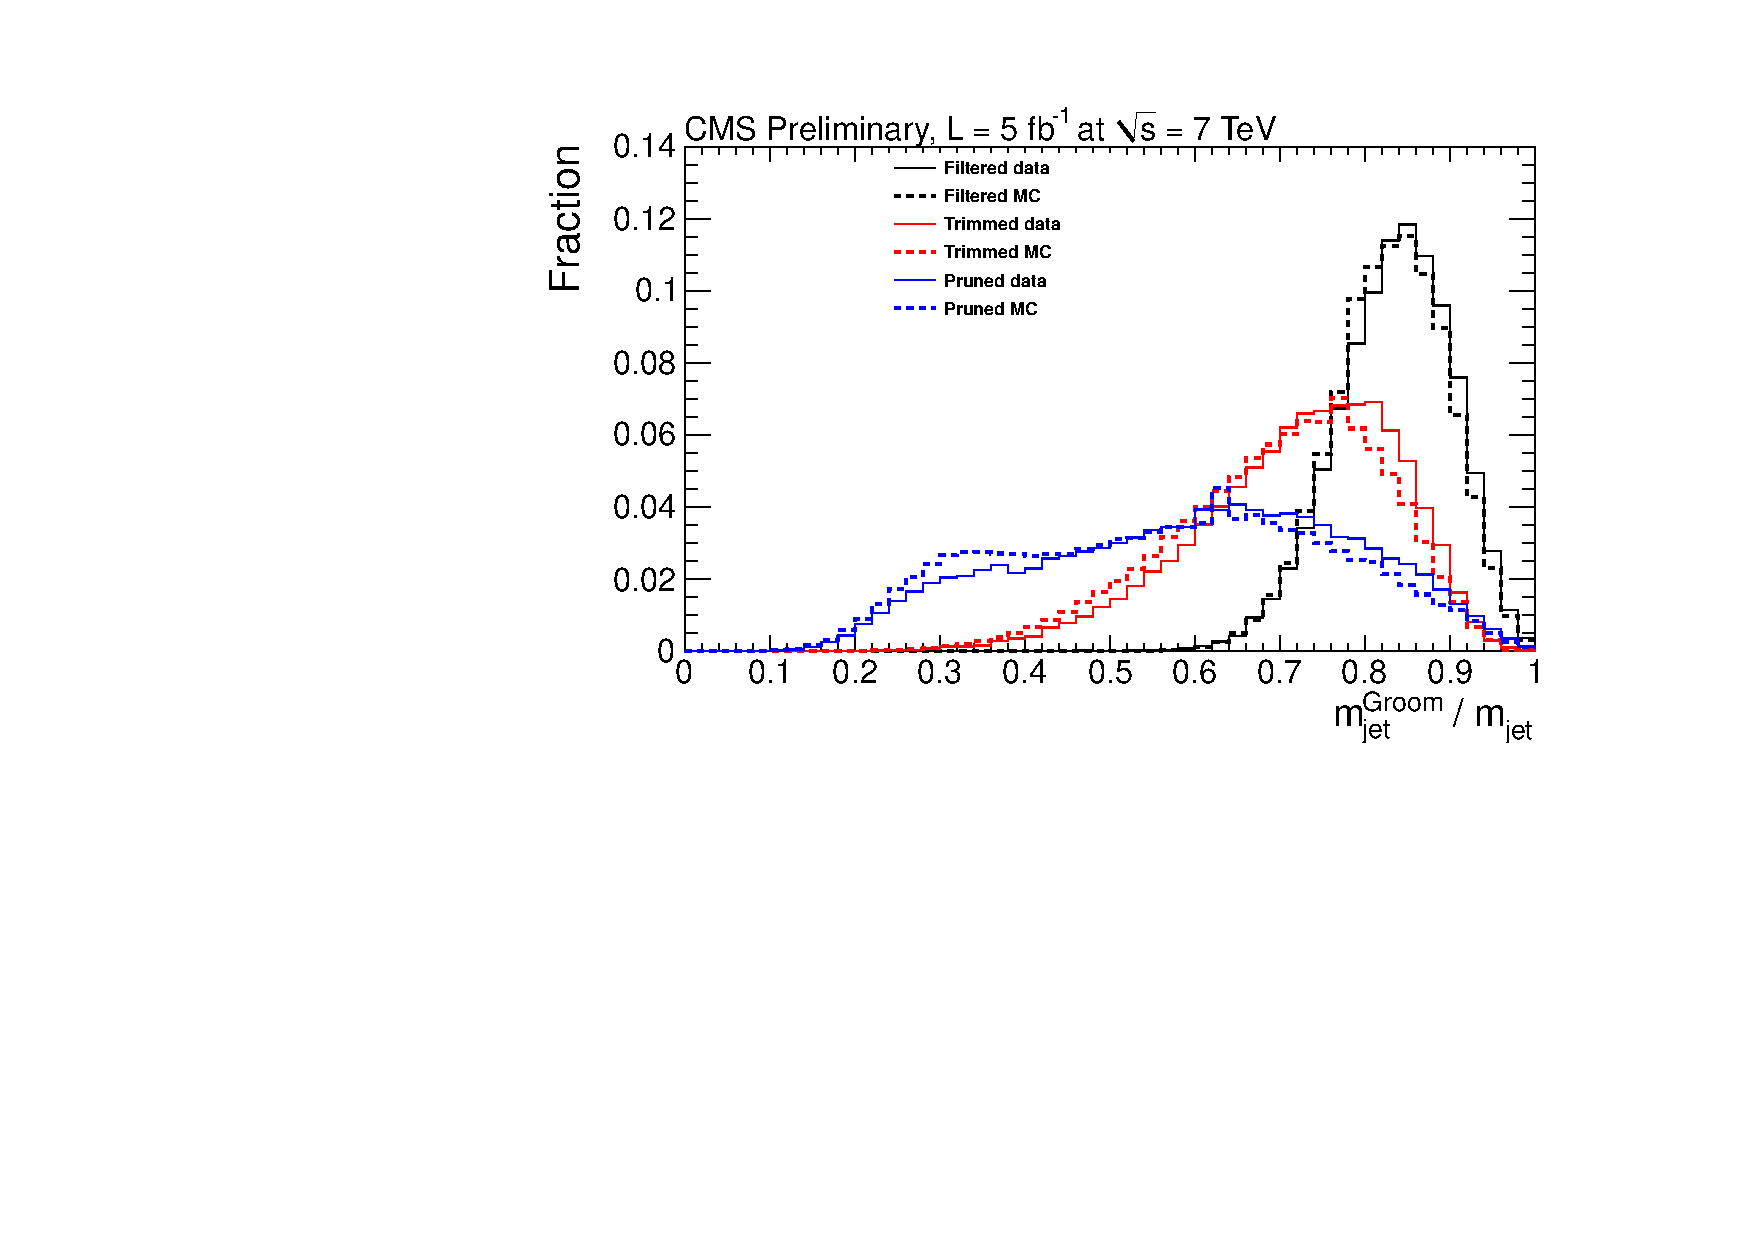
\includegraphics[width=0.95\textwidth]{figs/histAK7PtAvgVsMjetGroomOverReco_ratioPlots}
\caption{Distributions in differential probability for ratios of the jet mass of groomed jets
to their
corresponding ungroomed values, for both dijet data and \PYTHIA (tune Z2) MC
simulation, for the
three grooming techniques discussed in the text: 
(i) filtering (circles, peaking near $0.9$), 
(ii) trimming (squares, peaking near $0.75$), and 
(iii) pruning (triangles, more dispersed). 
\label{figs:histAK7PtAvgVsMjetGroomOverReco_ratioPlots}}
\end{figure}







\section{Event selection}
\label{sec:evsel_paper}

There are various selection criteria applied to the events to remove anomalous signals and noise from the objects for the measurement.
The events must have at least one good primary vertex as described in Sec.~\ref{sec:reconstruction}. 
Furthermore, beam backgrounds
are removed by requiring that events with at least 10 tracks 
have at least 25\% of the tracks satisfying high purity tracking requirements.
Finally, calorimeter noise is removed by timing and pulse shape selections on the signals
from the HB and HE calorimeters. 


For the dijet event selection, events are required to have at least two AK7 jets with
$\pt > 50$ \GeV and $|y| < 2.5$
and each jet must satisfy jet quality criteria \cite{particleflow}.

For the V+jets event selection,
reconstruction of W and Z bosons begins with the identification
and selection of charged leptons and MET described in the previous 
section.  Given the unique signature of a highly boosted vector 
boson recoiling from jets, a minimal selection is sufficient to 
identify highly pure samples of V+jets events. The background is dominated by $\mathrm{t\bar{t}}$ event (and in lower extent from single top events) in the W+jet topology, while in the Z$(\ell\ell)$+jet ($\ell=$ e,$\mu$) analysis the additional constraint on the di-lepton 
mass removes almost completely these backgrounds.  

Candidate \ZtoLL\ decays are reconstructed by combining 
isolated electrons and muons and requiring the dilepton invariant 
mass to satisfy $80<M_{\ell\ell}<100\GeV$.  

Candidate \WtoLN\ decays are identifed primarily by the topology
of a single isolated lepton with high $p_T$ and additional missing energy, with the selection described above.  The
transverse momentum \ptW\ and mass \mtW\ of the W candidate are obtained combining the lepton and the MET transverse four-momomenta components.

The jet mass analysis in V+ jet event is carried on in a boosted kinematic regime, namely $\pt $(V)$> 120$ GeV. We further require the leading jet in the event (independently for each clustering algorithm and jet radius) to have $\pt >$ 125 GeV.
Simply requiring a boosted regime, in addition to the tight isolation cuts on the leptons, is very effective to suppress the QCD background.
In the \WtoLN\ +jet analysis, further QCD rejection is achieved by requiring MET $>$ 50 GeV and $M_T$(W)$>$ 50 GeV.

Figure~\ref{fig:Vjetpt} shows the $p_T$ distribution for Z and W plus jet events for the leading AK7 jet after the selection described above has been applied. 

\begin{figure}[htbp]
\centering
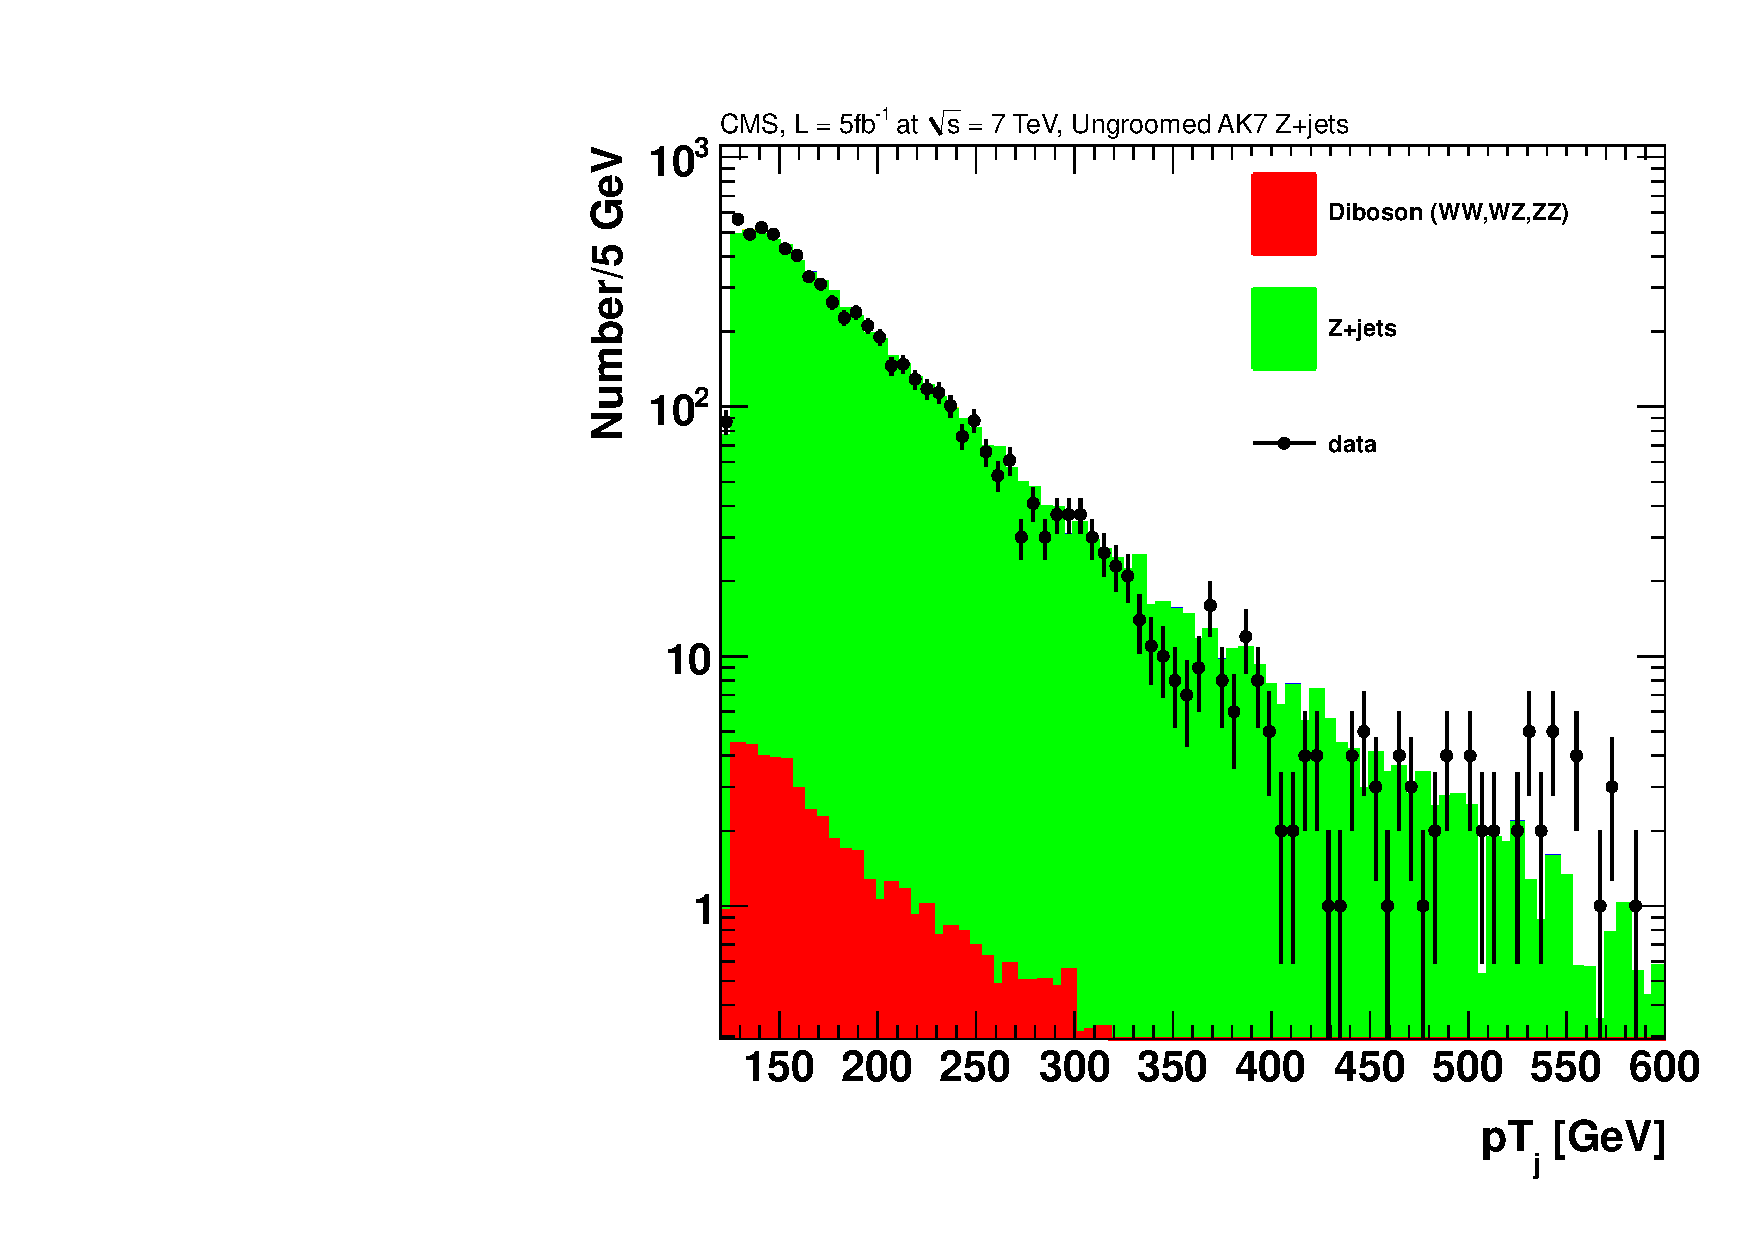
\includegraphics[width=0.495\textwidth]{figs/jetptZ_ak7.pdf}
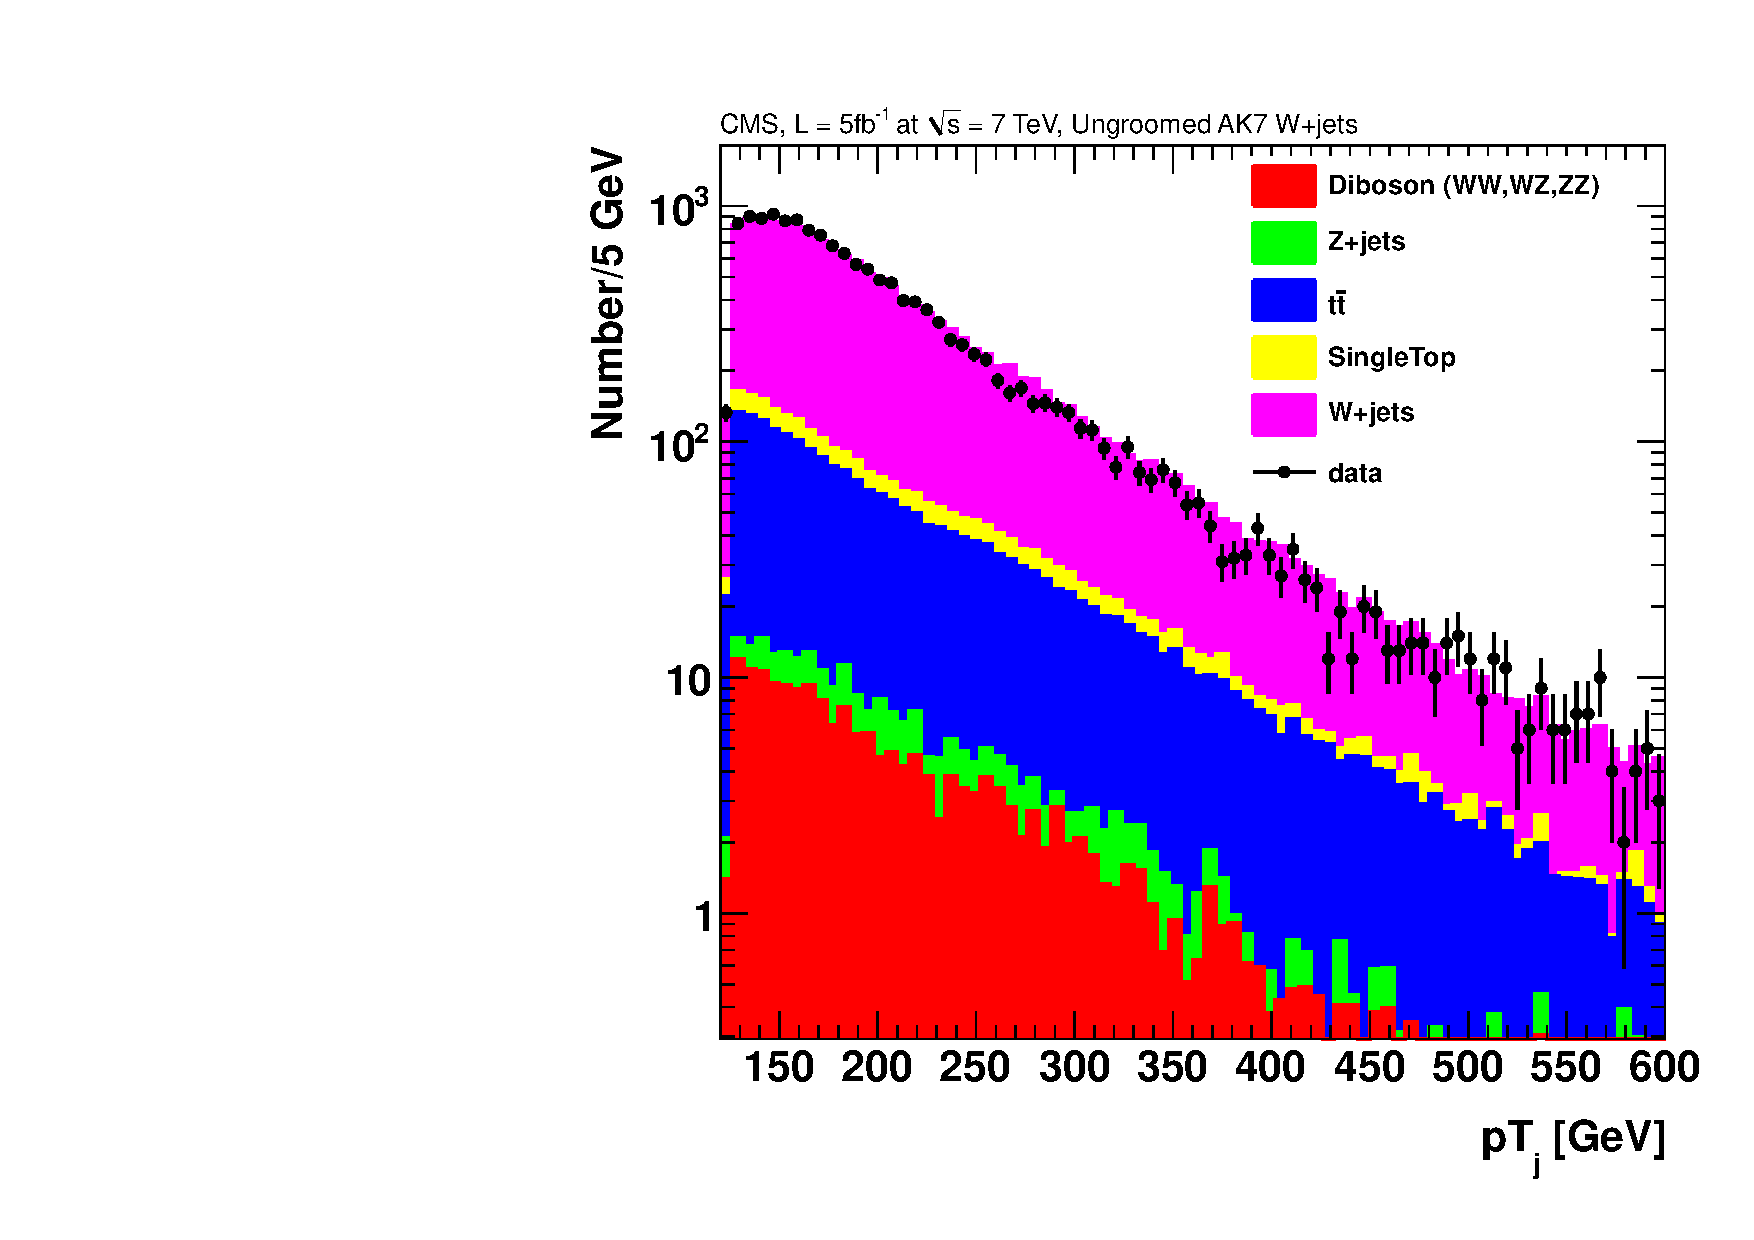
\includegraphics[width=0.495\textwidth]{figs/jetptW_ak7.pdf}
\caption{$p_T$ distribution for the leading AK7 jet in Z and W plus jet event passing the selection criteria.
\label{fig:Vjetpt}}
\end{figure}


After the selection, the Z+jet sample has a purity of about 99\%, with 1\% contamination form di-boson events. The W+jet sample is about 82\% pure, with backgrounds from $\mathrm{t\bar{t}}$ events (13\%), single top (3\%), di-boson and Z plus jets (1\% each). These backgrounds are subtracted based on their MC prediction from the final jet mass distributions before doing the unfolding procedure.
 



\section{Data Correction}

\label{sec:unfolding_paper}
The measured spectrum of a physical observable, like the jet mass distribution, is usually distorted by	detector effects, such as finite resolution and limited acceptance. Moreover, in this analysis the chosen bin size is comparable to the resolution, so there is a significant migration of events generated in one jet bin mass and ending up in a different bin of reconstructed jet mass. A comparison of the measured mass spectrum with that predicted at generator level requires that we remove these effects to obtain the true underlying mass spectrum. There are several possible ways to achieve the unfolding of detector effects on measured spectra. We use an unfolding procedure described by G.~D.~Agostini in~\cite{agostini}. Repeated application of Bayes theorem is used 
to invert the response matrix. Regularization is achieved by stopping iterations before reaching the ``true'' (but wildly fluctuating) inverse. The regularization parameter is just the number of iterations.
 In principle, this has to be tuned to prevent the statistical fluctuations being interpreted as structure in the true distribution, according to the sample statistics and binning. In practice, the results are fairly insensitive to the precise setting used and four iterations are usually sufficient. A trivial bin-by-bin unfolding technique is used as a cross check, and consistent results are observed where expected. 



\section{Systematics}
\label{sec:systematics}

The systematic uncertainties were investigated by comparing
the unfolded $m_{jet}$ distribution for each systematic
variation to the nominal value, which is taken from
\PYTHIA. 

The experimental uncertainties considered include  
the jet energy scale, estimated by raising and lowering the jet energy by the measured uncertainty as a function of jet $\pt$ and $\eta$, and the jet energy and angular resolution, estimated by increasing and decreasing the jet energy, $\eta$ and $\phi$ resolution by 10\%.
The nominal value chosen is 10\%, motivated by the observed difference between data and simulation in the jet energy resolution~\cite{citeJEC}, so the up and down variations 
correspond to 20\% and 0\% additional smearing with respect to the Monte Carlo, respectively. 
We also estimate an uncertainty associated with the pile-up simulated in the MC, estimated by increasing and decreasing the minimum bias cross section by 8\%. 

As theoretical uncertainty due to the parton showering model, we conservatively estimate it by comparing unfolded \MADGRAPH to unfolded \HERWIG and assigning the difference as a systematic uncertainty.

After these effects are investigated, it is found that the dominant uncertainty is
the difference in the parton showering model. All uncertainties are included in
the measurement. 



\section{Results}
\label{sec:vjetresults}

\label{sec:vjetresults}
%\clearpage

This section provides the probability density distributions as functions of
the mass of the leading jet in V+jet events. These distributions are
corrected for detector effects in the jet mass, and are compared to MC expectations
from \MADGRAPH (interfaced to \PYTHIA) and \HERWIG.  
The jet mass distributions are studied in different ranges of $\pt$
between $125$ and $450\GeV$, as given in Table~\ref{tab:ptBins}. 
(Just as in
the dijet results, $\pt$
is not corrected to the particle level.) For
jets reconstructed with the CA algorithm ($R=1.2$), we study only the
events with
$\pt>150\GeV$, which is most interesting for
heavy particle searches in the highly-boosted regime, where all decay
products are contained within $R=1.2$ jets~\cite{boostedHiggs}. 

For clarity, the distributions are also truncated at large mass values where few events are recorded.
 Jet-mass bins with relative uncertainties 
$>$ 100\% are also ignored to minimize overlap with more precise measurements in other $\pt$ bins.

%We report normalized cross-sections, i.e. $1/\sigma*(d\sigma/dM_J)$ in order to cancel luminosity dependence.
%We present normalized cross-sections, as defined in Eq.~\ref{eq:pdf_mjet_simple}.
%Both \MADGRAPH and \HERWIG are found to reproduce the data reasonably well: the agreement improves for large $\pt$, while, similarly to the dijet analysis, the modeling is poor at low mass. This region is usually of limited interest in new physics searches. % (that is also the most sensitive region to PU effects). %It is also interesting to observe that the more aggressive the grooming is, the more herwig seems to better reproduce the data than madgraph/pythia. 


%\subsection{Z$(\ell\ell)$+ jet Analysis}

Figures~\ref{figs:AK7ZmmInt1}--\ref{figs:AK7ZmmInt2} show mass
distributions for the leading AK7 jet accompanying a \Z boson in
$\Z(\ell\ell)$+jet events for the ungroomed, filtered, trimmed,
and pruned clustering of jets, respectively. Both \PYTHIA and
\HERWIG show good agreement with data for all $\pt$ bins, but
especially so for $\pt >$ 300 \GeV. As in the case of the dijet
analysis, the data at small jet mass are not modeled satisfactorily, but
show modest improvement after applying the grooming procedures.
To investigate several popular choices of jet grooming at CMS,
Figs.~\ref{figs:prunedZmmInt1}--\ref{figs:prunedZmmInt2} show the
distributions in $m_J$ for pruned CA8 and filtered CA12 jets in {\Z}$+$jet
events.  For groomed CA jets, both  \PYTHIA and \HERWIG provide
good agreement with the data, with some possible inconsistency for
$m_J< 20 \GeV$ and at large $m_J$ for $\pt< 300 \GeV$ for the ungroomed and
filtered jets.
Figures~\ref{figs:AK7WmnInt1}--\ref{figs:AK7WmnInt2} show the
corresponding distributions for the mass of the leading jet
accompanying the \PW~boson for AK7 jets in \PW$(\ell\nu_\ell)$+jet
events for the ungroomed, filtered, trimmed, and pruned clustering
algorithms, and
Figs.~\ref{figs:prunedWmnInt1}--\ref{figs:prunedWmnInt2} show the
distributions for pruned CA8 and filtered CA12 jets.
For CA8 and CA12 jets, only particular grooming algorithms and $\pt$ bins are chosen for illustration.
The MC simulation shows good agreement with data, just as observed for 
{\Z}$+$jet events. 


\begin{figure}[!htb]
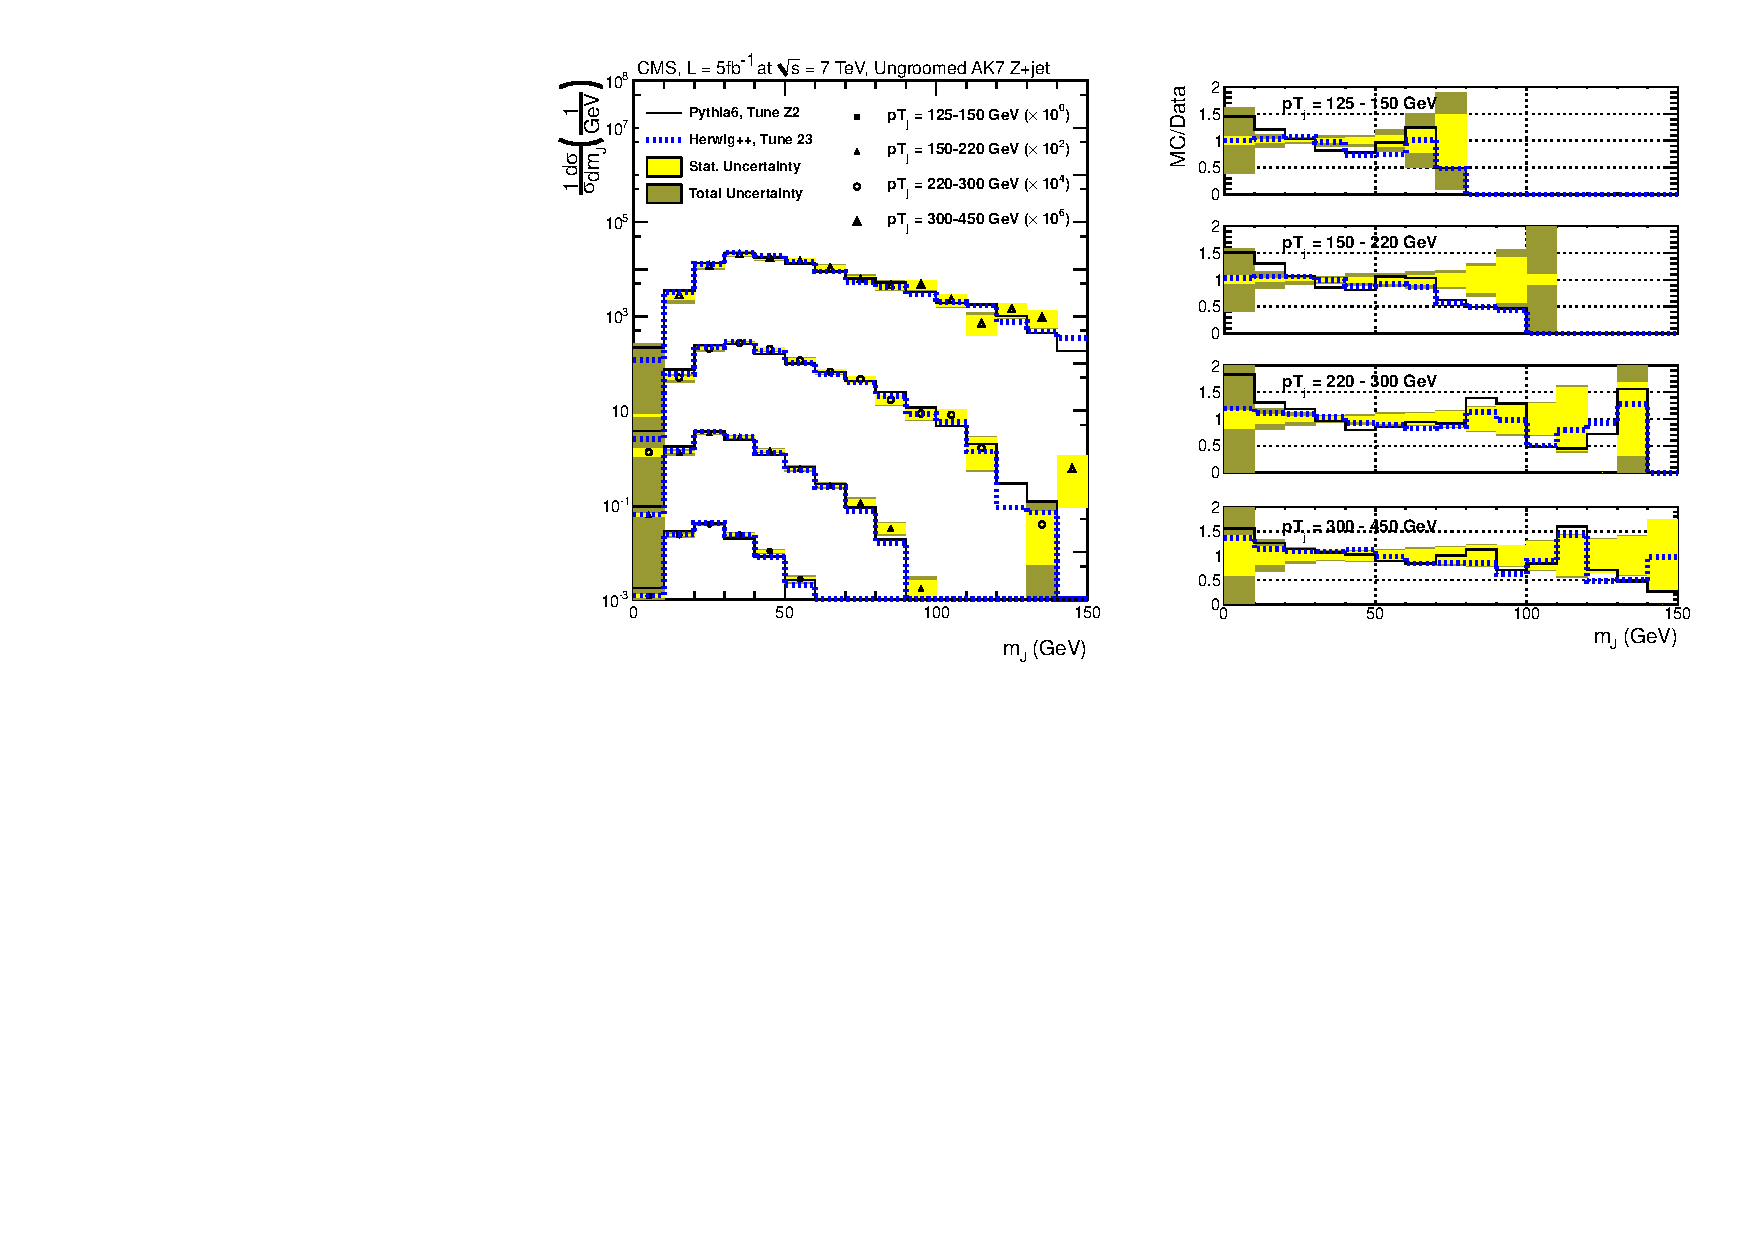
\includegraphics[width=0.99\textwidth]{figs/Zll/jetmassunf_ak7_log_Z.pdf}
\caption{Unfolded, ungroomed AK7 $m_J$ distribution for $\Z(\ell\ell)$+jet events. The data (black symbols) are compared to MC expectations from {\MADGRAPH}+\PYTHIA (solid lines) and \HERWIG (dotted lines) on the left. The ratio of MC to data is given on the right.
The statistical uncertainty is shown in light shading, and the total uncertainty in dark shading.}
\label{figs:AK7ZmmInt1}
\end{figure}

\begin{figure}[!htb]
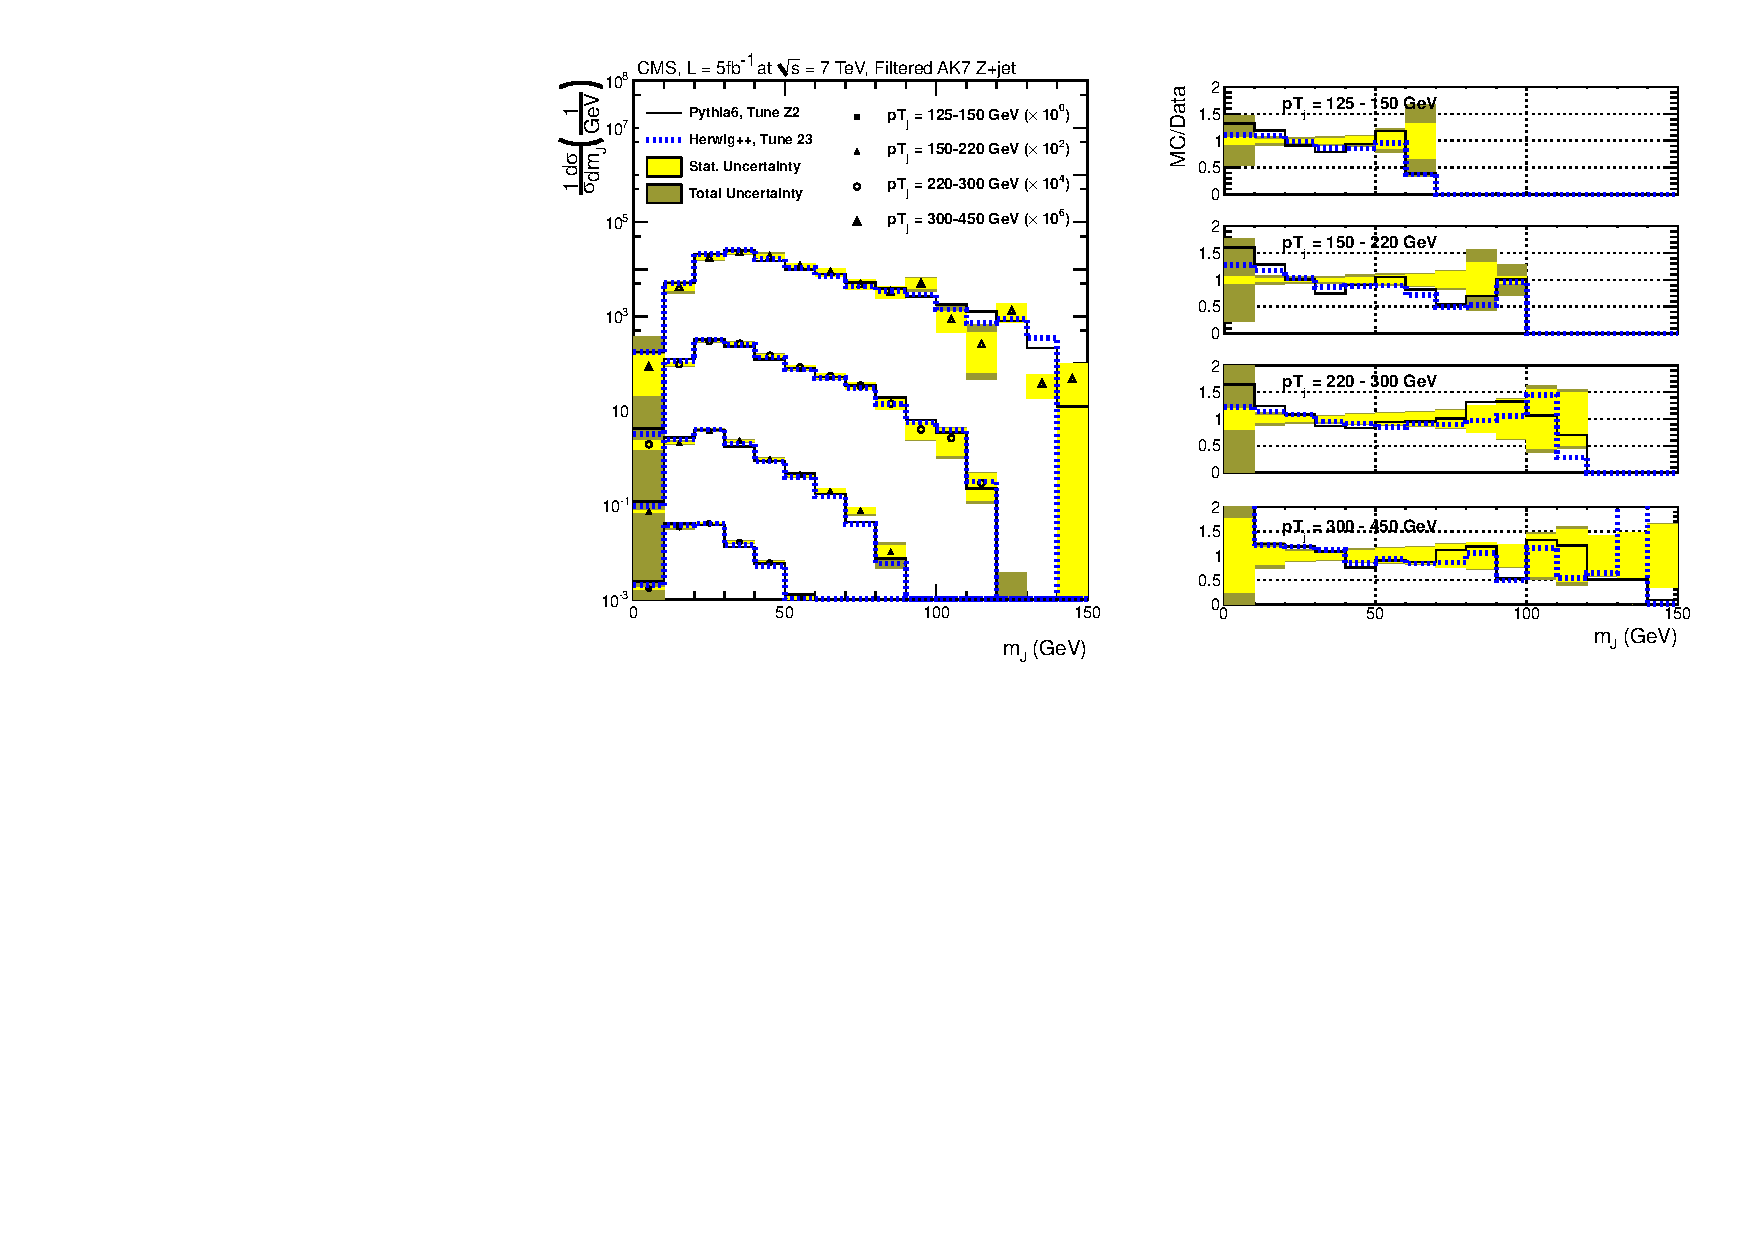
\includegraphics[width=0.99\textwidth]{figs/Zll/jetmassunf_ak7ft_log_Z.pdf}
\caption{Unfolded AK7 filtered $m_J$ distribution for $\Z(\ell\ell)$+jet events. The data (black symbols) are compared to MC expectations from {\MADGRAPH}+\PYTHIA (solid lines) and \HERWIG (dotted lines) on the left. The ratio of MC to data is given on the right.
The statistical uncertainty is shown in light shading, and the total uncertainty in dark shading.}
\label{figs:AK7ZmmInt3}
\end{figure}

\begin{figure}[!htb]
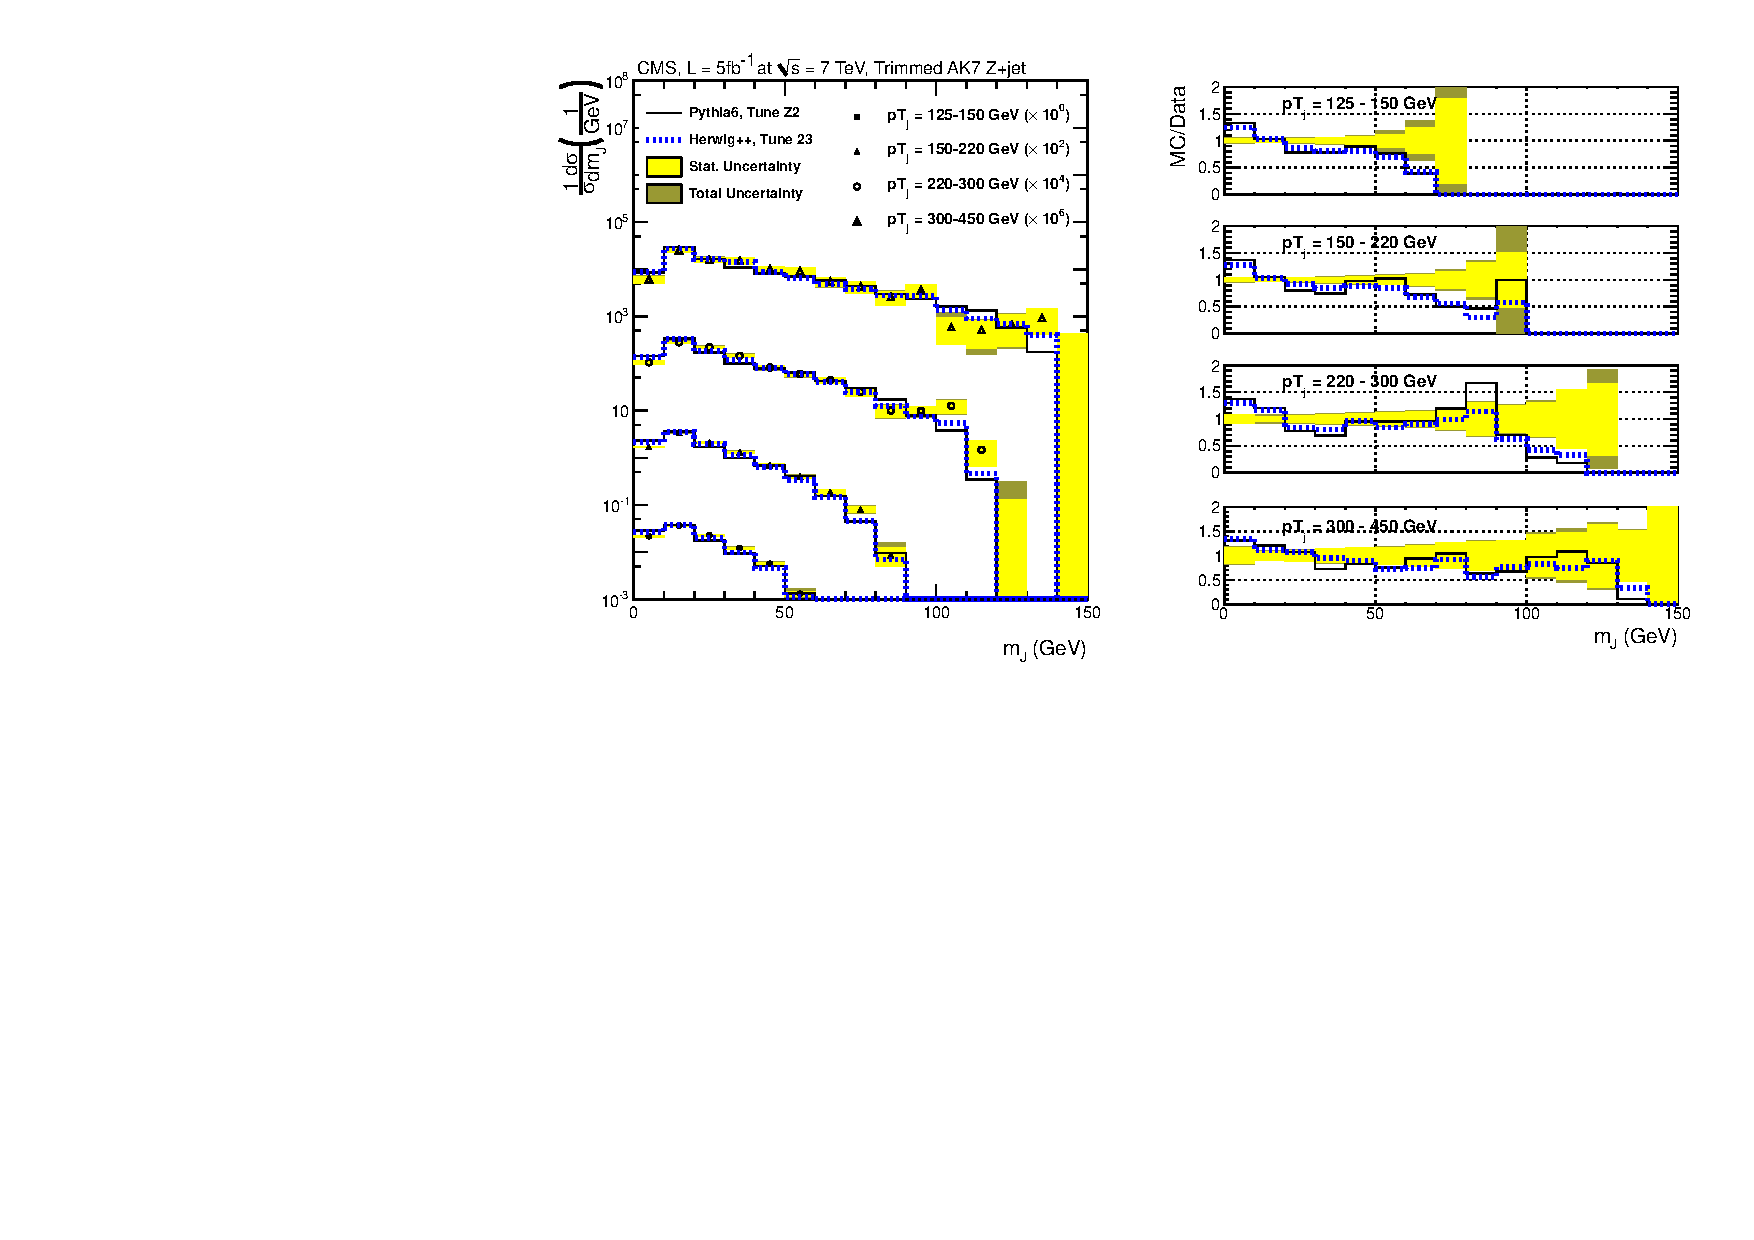
\includegraphics[width=0.99\textwidth]{figs/Zll/jetmassunf_ak7tr_log_Z.pdf}
\caption{Unfolded AK7 trimmed $m_J$ distribution for $\Z(\ell\ell)$+jet events. The data (black symbols) are compared to MC expectations from {\MADGRAPH}+\PYTHIA (solid lines) and \HERWIG (dotted lines) on the left. The ratio of MC to data is given on the right.
The statistical uncertainty is shown in light shading, and the total uncertainty in dark shading.}
\label{figs:AK7ZmmInt4}
\end{figure}

\begin{figure}[!htb]
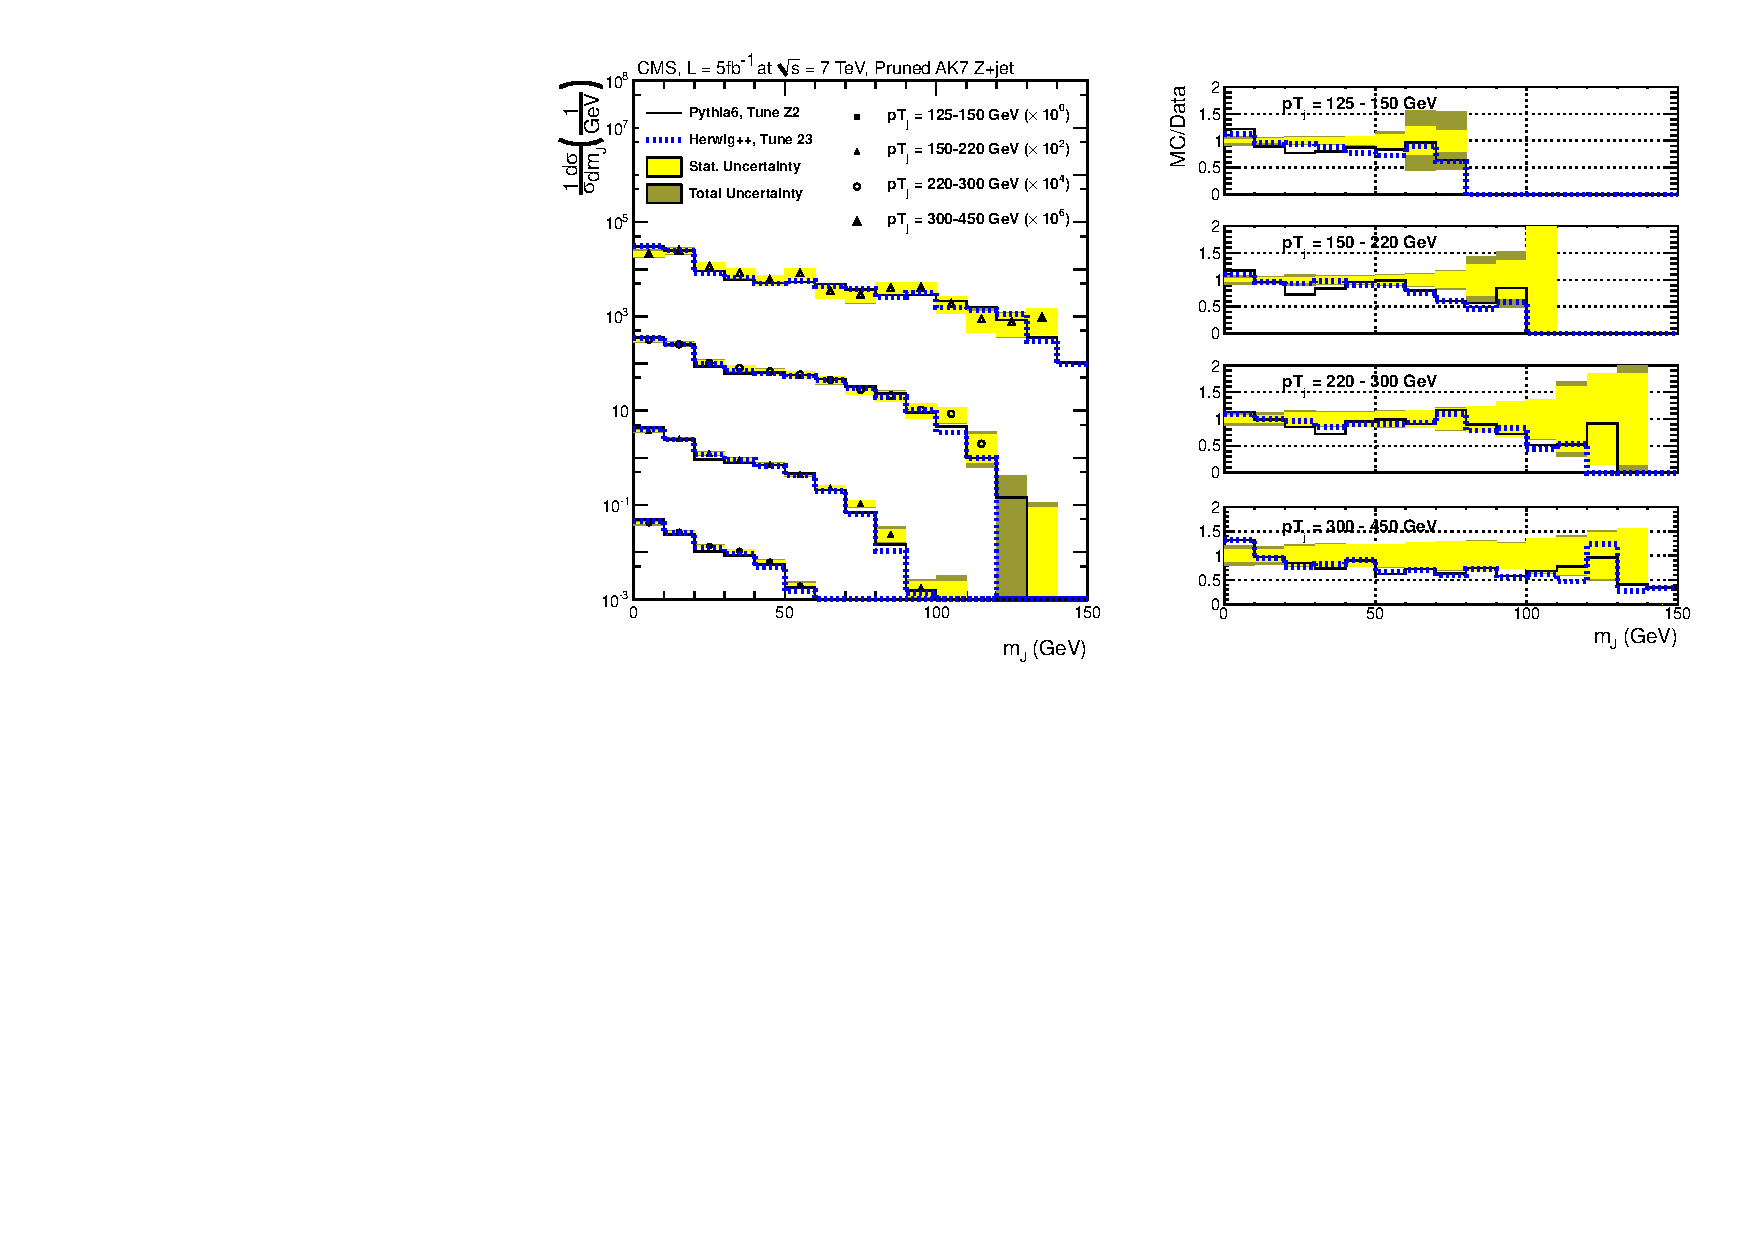
\includegraphics[width=0.99\textwidth]{figs/Zll/jetmassunf_ak7pr_log_Z.pdf}
\caption{Unfolded AK7 pruned $m_J$ distribution for $\Z(\ell\ell)$+jet events. The data (black symbols) are compared to MC expectations from {\MADGRAPH}+\PYTHIA (solid lines) and \HERWIG (dotted lines) on the left. The ratio of MC to data is given on the right.
The statistical uncertainty is shown in light shading, and the total uncertainty in dark shading.}
\label{figs:AK7ZmmInt2}
\end{figure}

\begin{figure}[!htb]
\centering
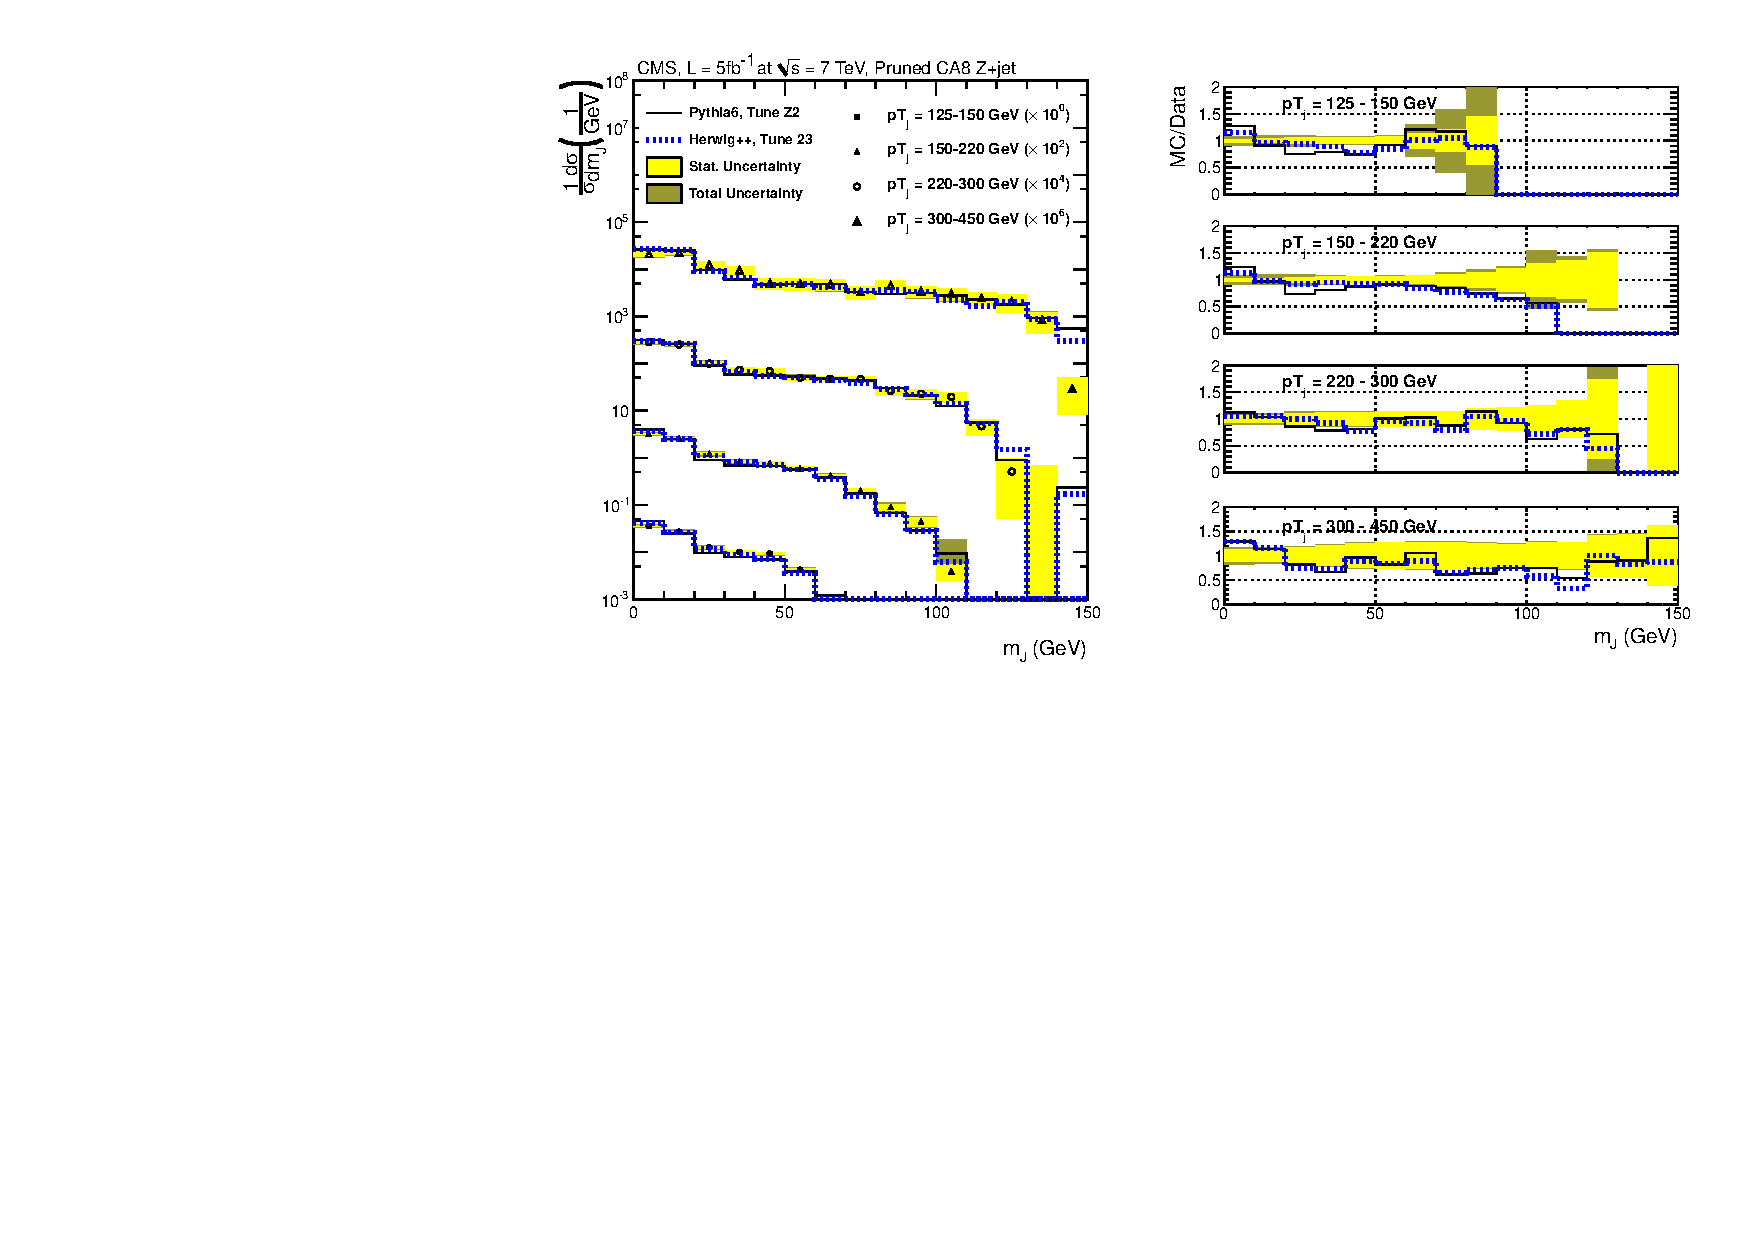
\includegraphics[width=0.99\textwidth]{figs/Zll/jetmassunf_ca8pr_log_Z.pdf}
\caption{Unfolded CA8 pruned $m_J$ distribution for $\Z(\ell\ell)$+jet events. The data (black symbols) are compared to MC expectations from {\MADGRAPH}+\PYTHIA (solid lines) and \HERWIG (dotted lines) on the left. The ratio of MC to data is given on the right.
The statistical uncertainty is shown in light shading, and the total uncertainty in dark shading.}
\label{figs:prunedZmmInt1}
\end{figure}

\begin{figure}[!htb]
\centering
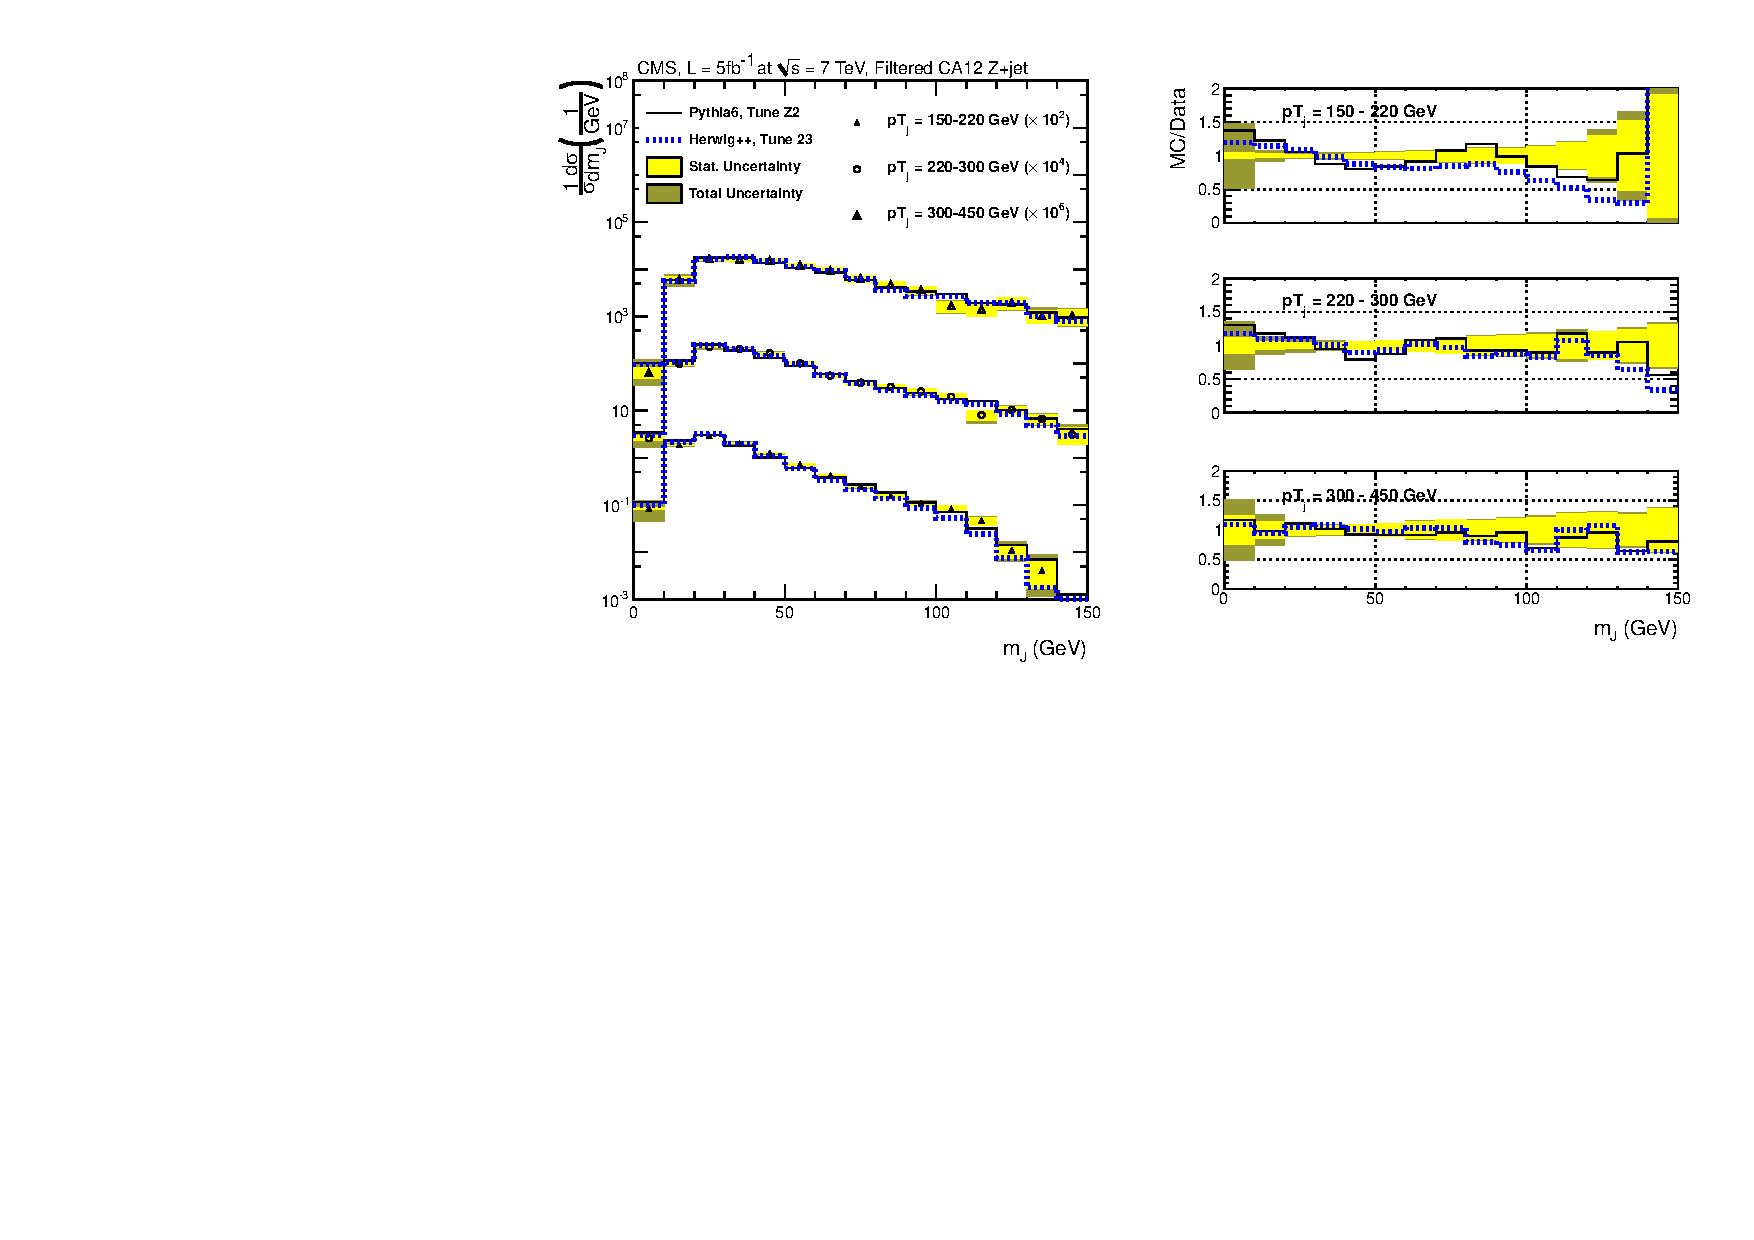
\includegraphics[width=0.99\textwidth]{figs/Zll/jetmassunf_ca12ft_log_Z.pdf}
\caption{Unfolded CA12 filtered $m_J$ distribution for $\Z(\ell\ell)$+jet events. The data (black symbols) are compared to MC expectations from {\MADGRAPH}+\PYTHIA (solid lines) and \HERWIG (dotted lines) on the left. The ratio of MC to data is given on the right.
The statistical uncertainty is shown in light shading, and the total uncertainty in dark shading.}
\label{figs:prunedZmmInt2}
\end{figure}


\clearpage


%\subsection{W$(\ell\nu)$ +jet Analysis}

%Fig.~\ref{figs:AK7WmnInt1}-\ref{figs:AK7WmnInt4} shows the $m_J$ distribution for AK7 jets in W$(\ell\nu)$ +jet events, for the different clustering algorithm studied: ungroomed, pruned, trimmed, and filtered respectively.
%Fig.~\ref{figs:prunedWmnInt1}-\ref{figs:prunedWmnInt2} shows the $m_J$ distribution for pruned CA8 and filtered CA12 jets in W$(\ell\nu)$ +jet events.
%The simulation has a good agreement with data: similar observations as the ones reported for the Z+jet events apply also here.

\begin{figure}[!htb]
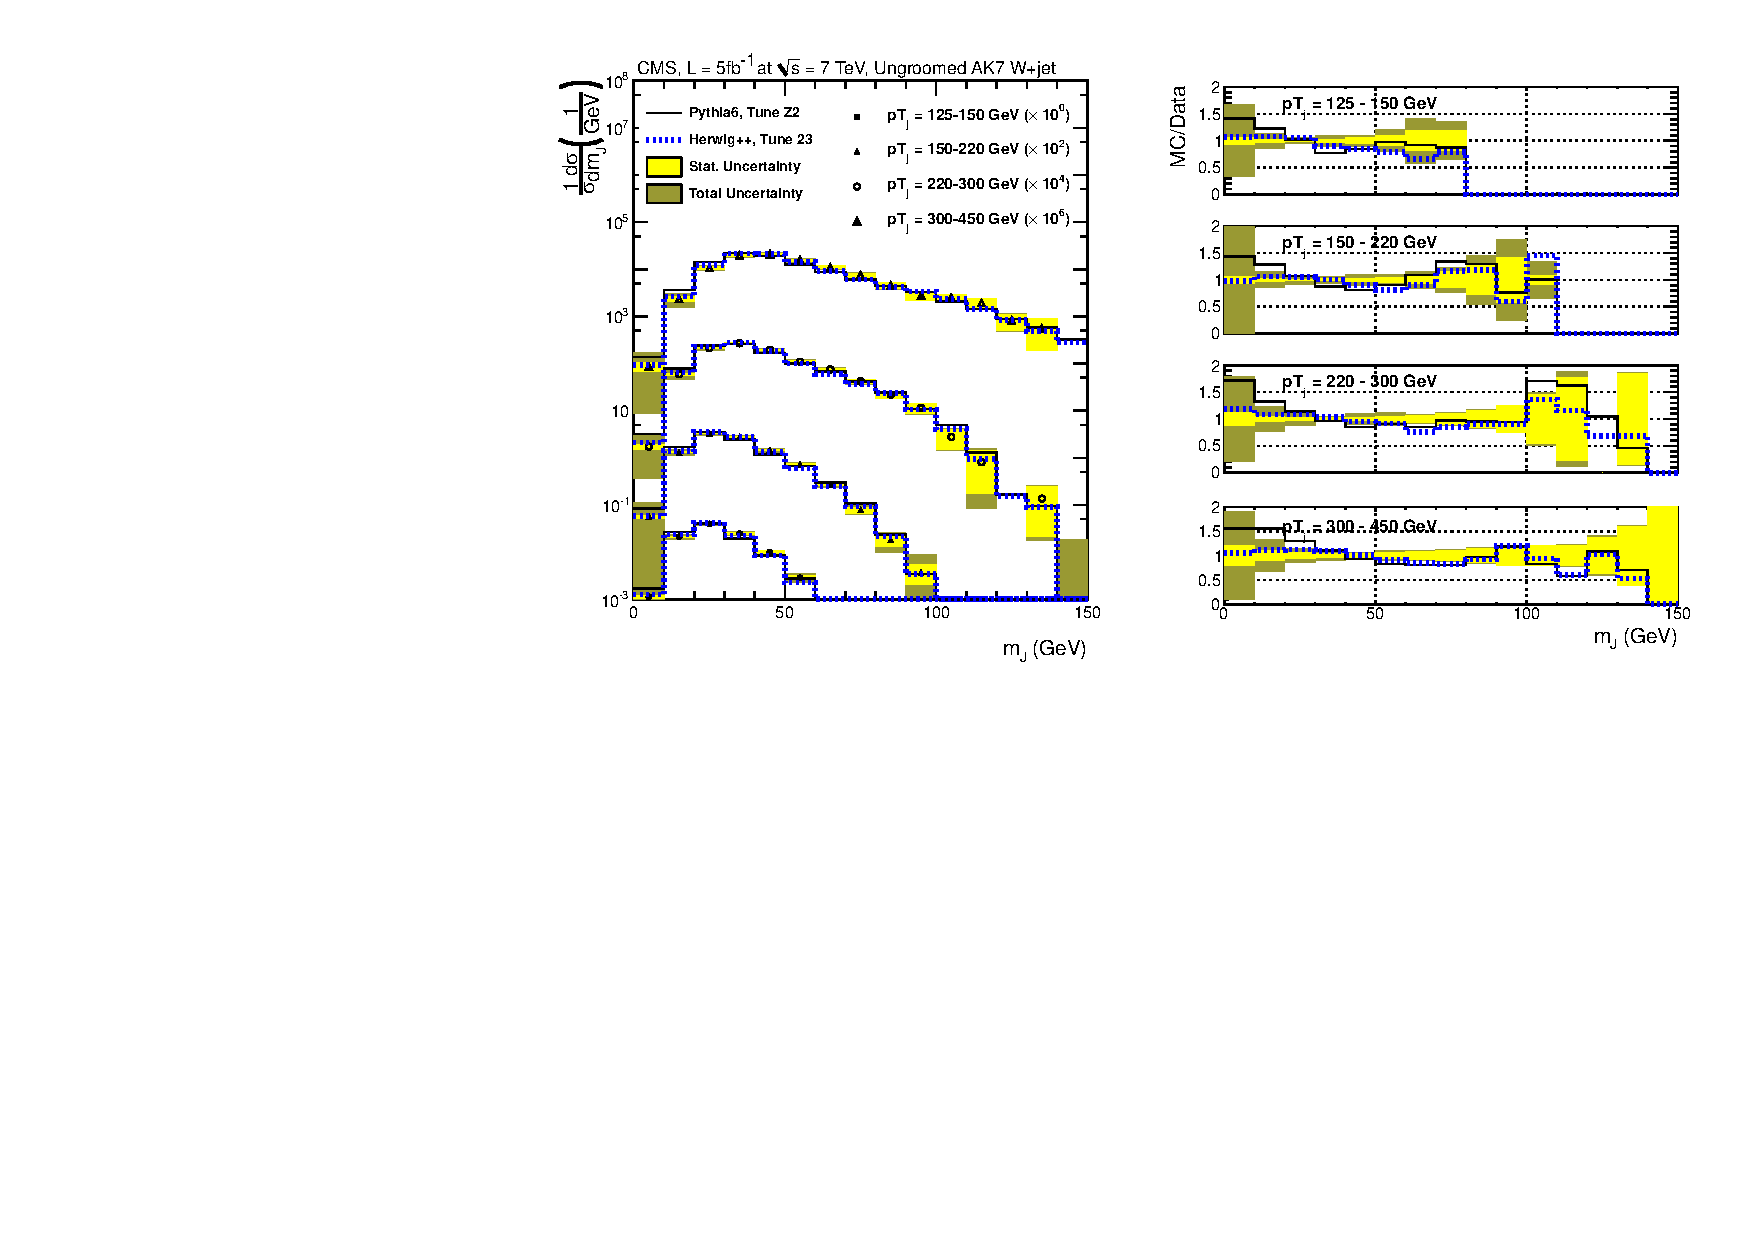
\includegraphics[width=0.99\textwidth]{figs/Wln/jetmassunf_ak7_log_W.pdf}
\caption{Distributions in $m_J$ for unfolded, ungroomed AK7 jets in  \PW$(\ell\nu_\ell)$+jet events. The data (black symbols) are compared to MC expectations from {\MADGRAPH}+\PYTHIA (solid lines) and \HERWIG (dotted lines) on the left. The ratios of MC to data are given on the right.
The statistical uncertainty is shown in light shading, and the total uncertainty in dark shading.}
\label{figs:AK7WmnInt1}
\end{figure}

\begin{figure}[!htb]
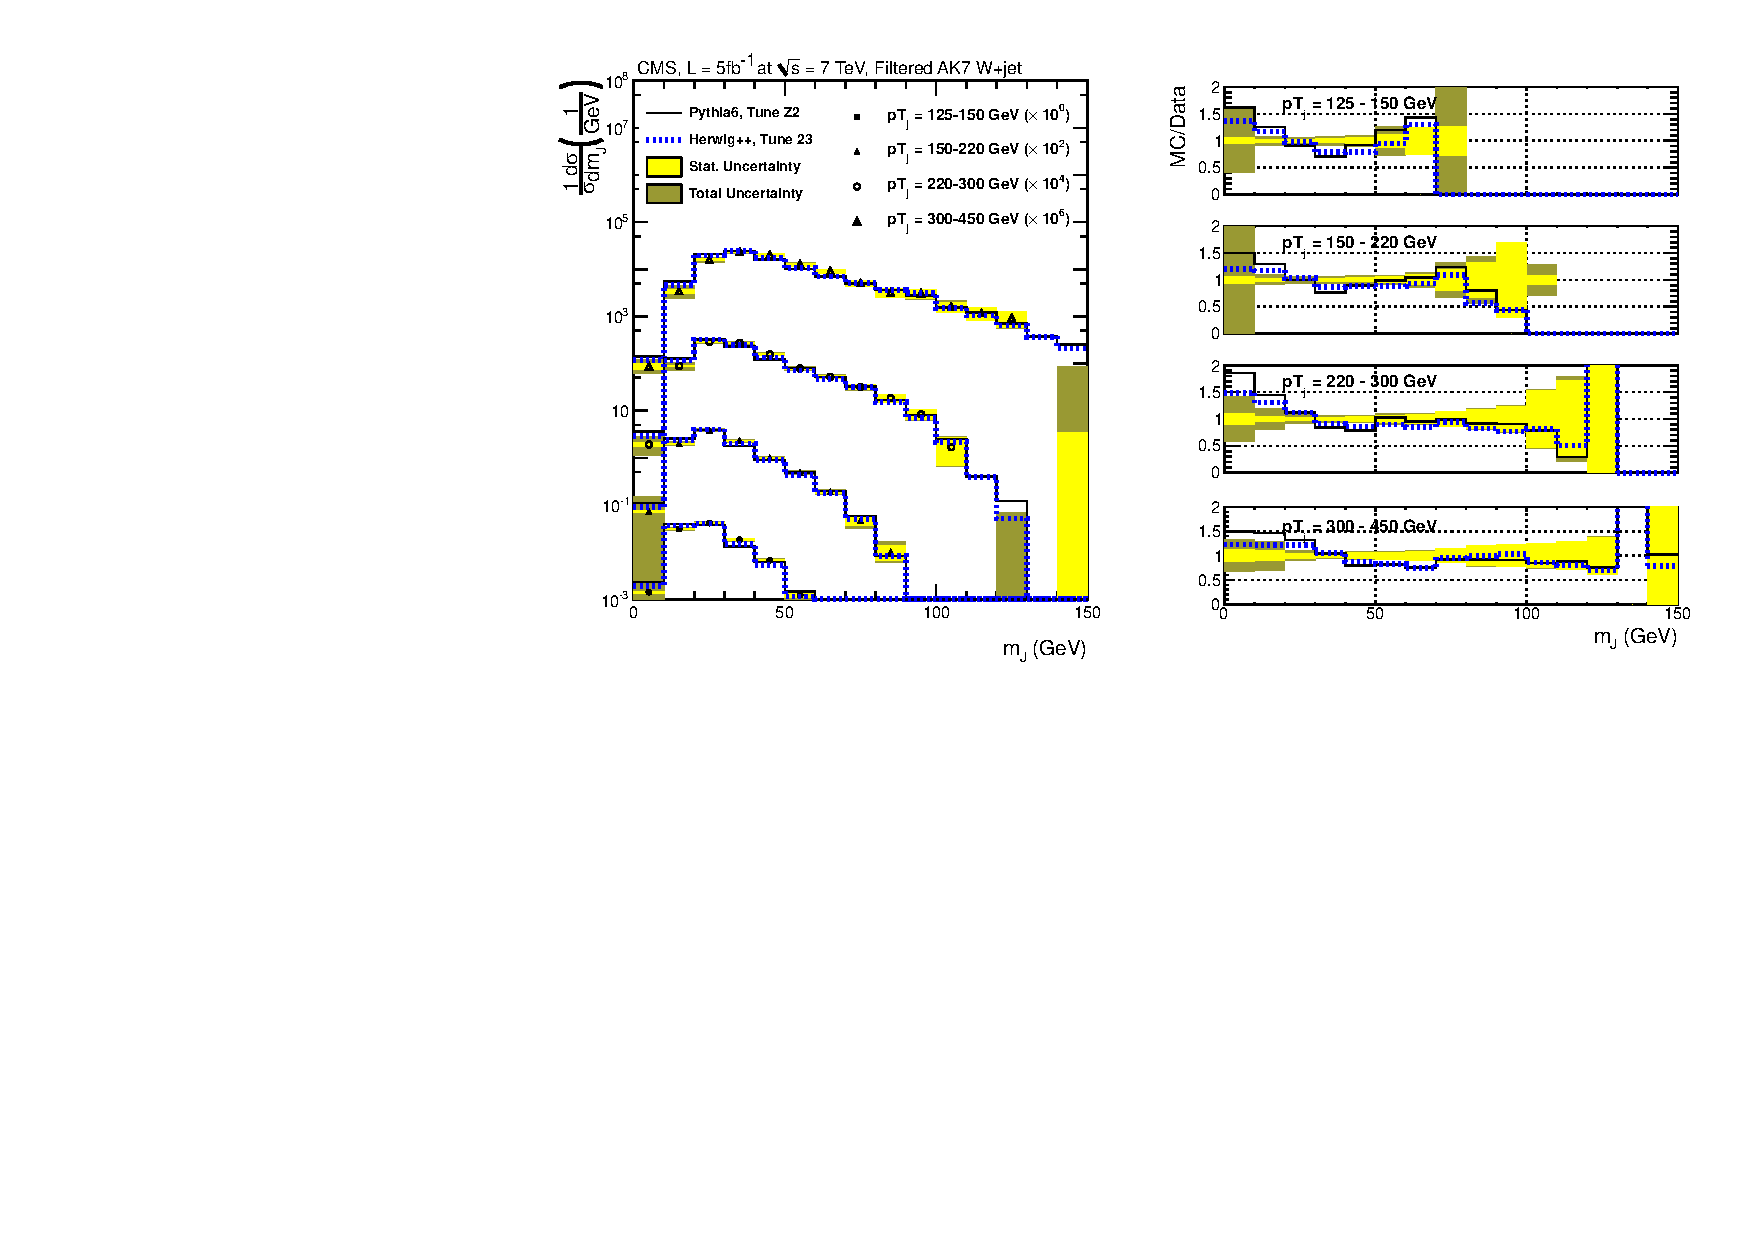
\includegraphics[width=0.99\textwidth]{figs/Wln/jetmassunf_ak7ft_log_W.pdf}
\caption{Distributions in $m_J$ for unfolded, filtered AK7 jets in \PW$(\ell\nu_\ell)$+jet events. The data (black symbols) for different bins in $\pt$ are compared to MC expectations from {\MADGRAPH}+\PYTHIA (solid lines) and \HERWIG (dotted lines) on the left. The ratios of MC to data are given on the right.
The statistical uncertainty is shown in light shading, and the total uncertainty in dark shading.}
\label{figs:AK7WmnInt3}
\end{figure}

\begin{figure}[!htb]
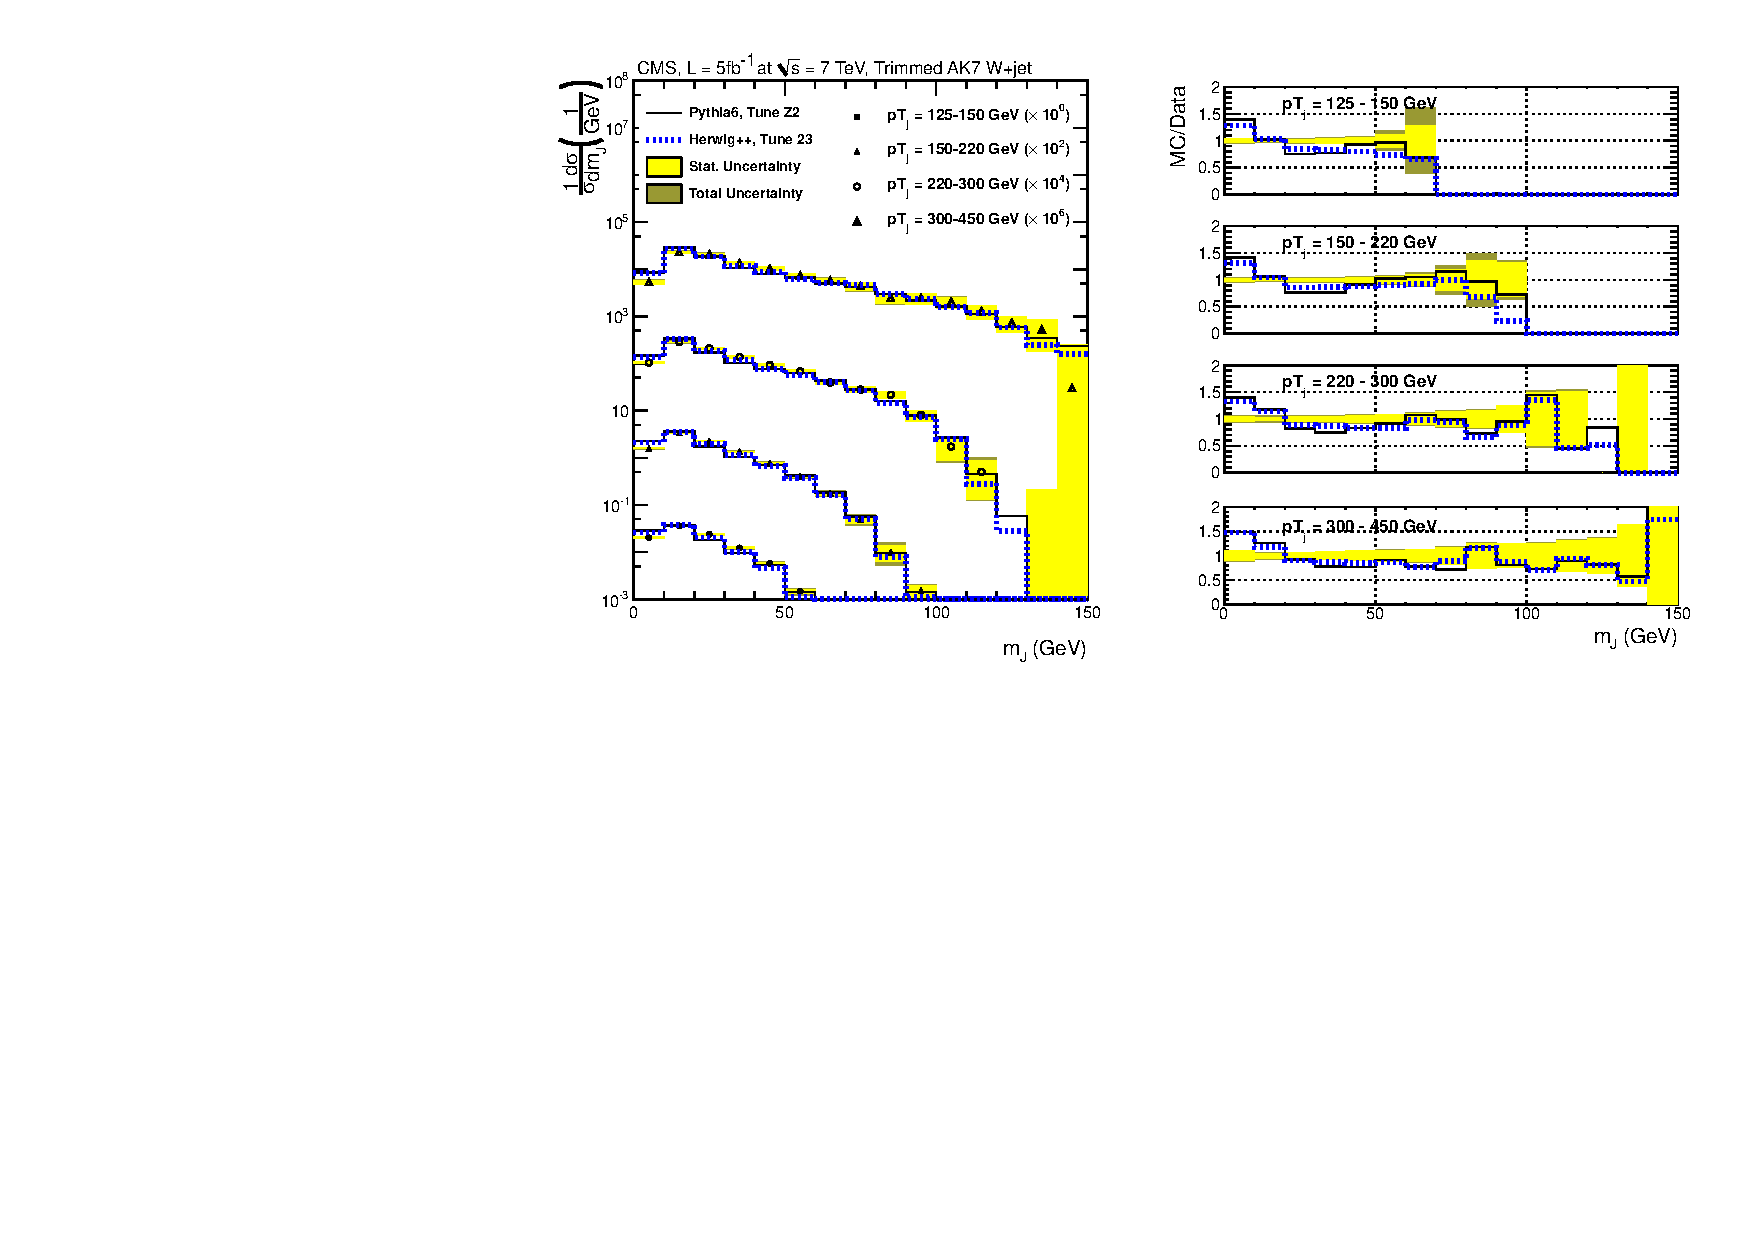
\includegraphics[width=0.99\textwidth]{figs/Wln/jetmassunf_ak7tr_log_W.pdf}
\caption{Distributions in $m_J$ for unfolded, trimmed AK7 jets in \PW$(\ell\nu_\ell)$+jet events. The data (black symbols) for different bins in $\pt$ are compared to MC expectations from {\MADGRAPH}+\PYTHIA (solid lines) and \HERWIG (dotted lines) on the left. The ratios of MC to data are given on the right.
The statistical uncertainty is shown in light shading, and the total uncertainty in dark shading.}
\label{figs:AK7WmnInt4}
\end{figure}

\begin{figure}[!htb]
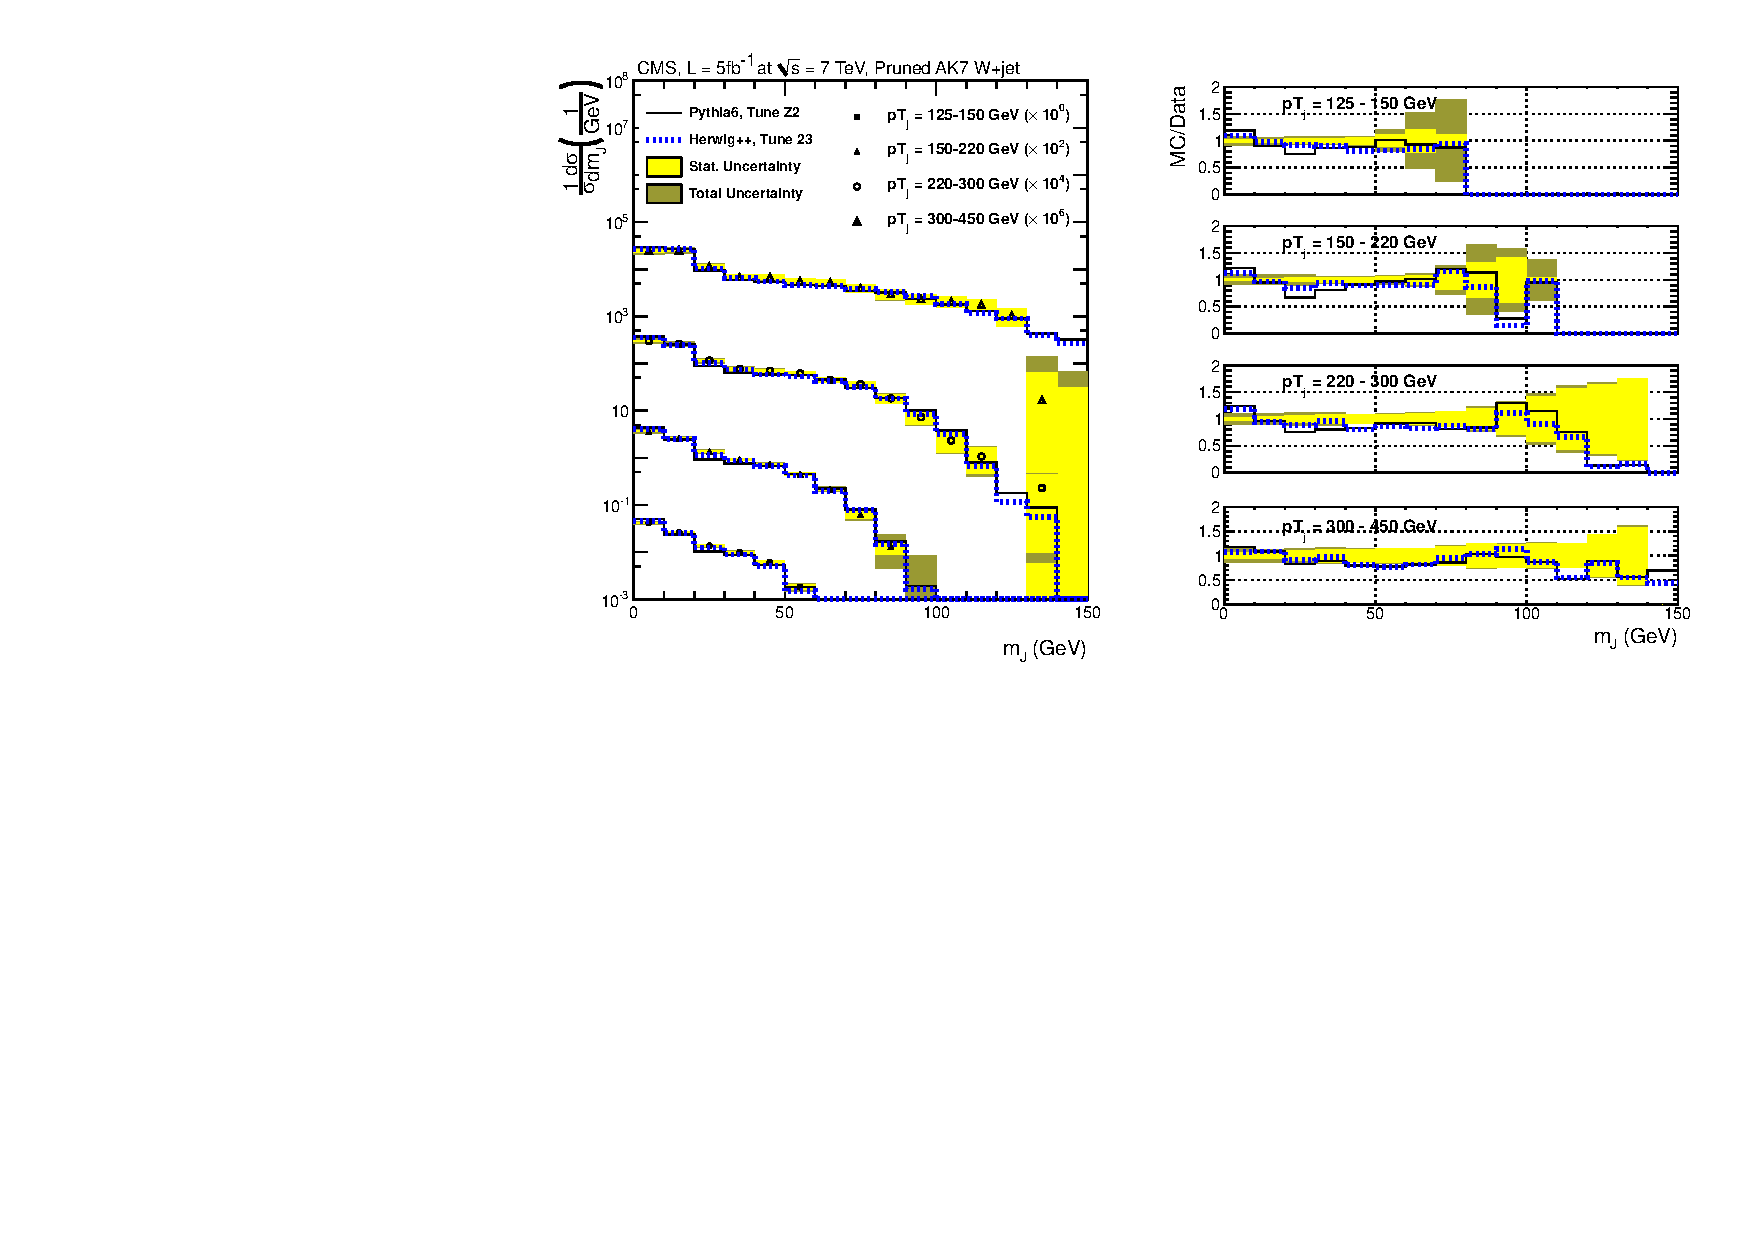
\includegraphics[width=0.99\textwidth]{figs/Wln/jetmassunf_ak7pr_log_W.pdf}
\caption{Distributions in $m_J$ for unfolded, pruned AK7 jets in \PW$(\ell\nu_\ell)$+jet events. The data (black symbols) for different bins in $\pt$ are compared to MC expectations from {\MADGRAPH}+\PYTHIA (solid lines) and \HERWIG (dotted lines) on the left. The ratios of MC to data are given on the right.
The statistical uncertainty is shown in light shading, and the total uncertainty in dark shading.}
\label{figs:AK7WmnInt2}
\end{figure}

\begin{figure}[!htb]
\centering
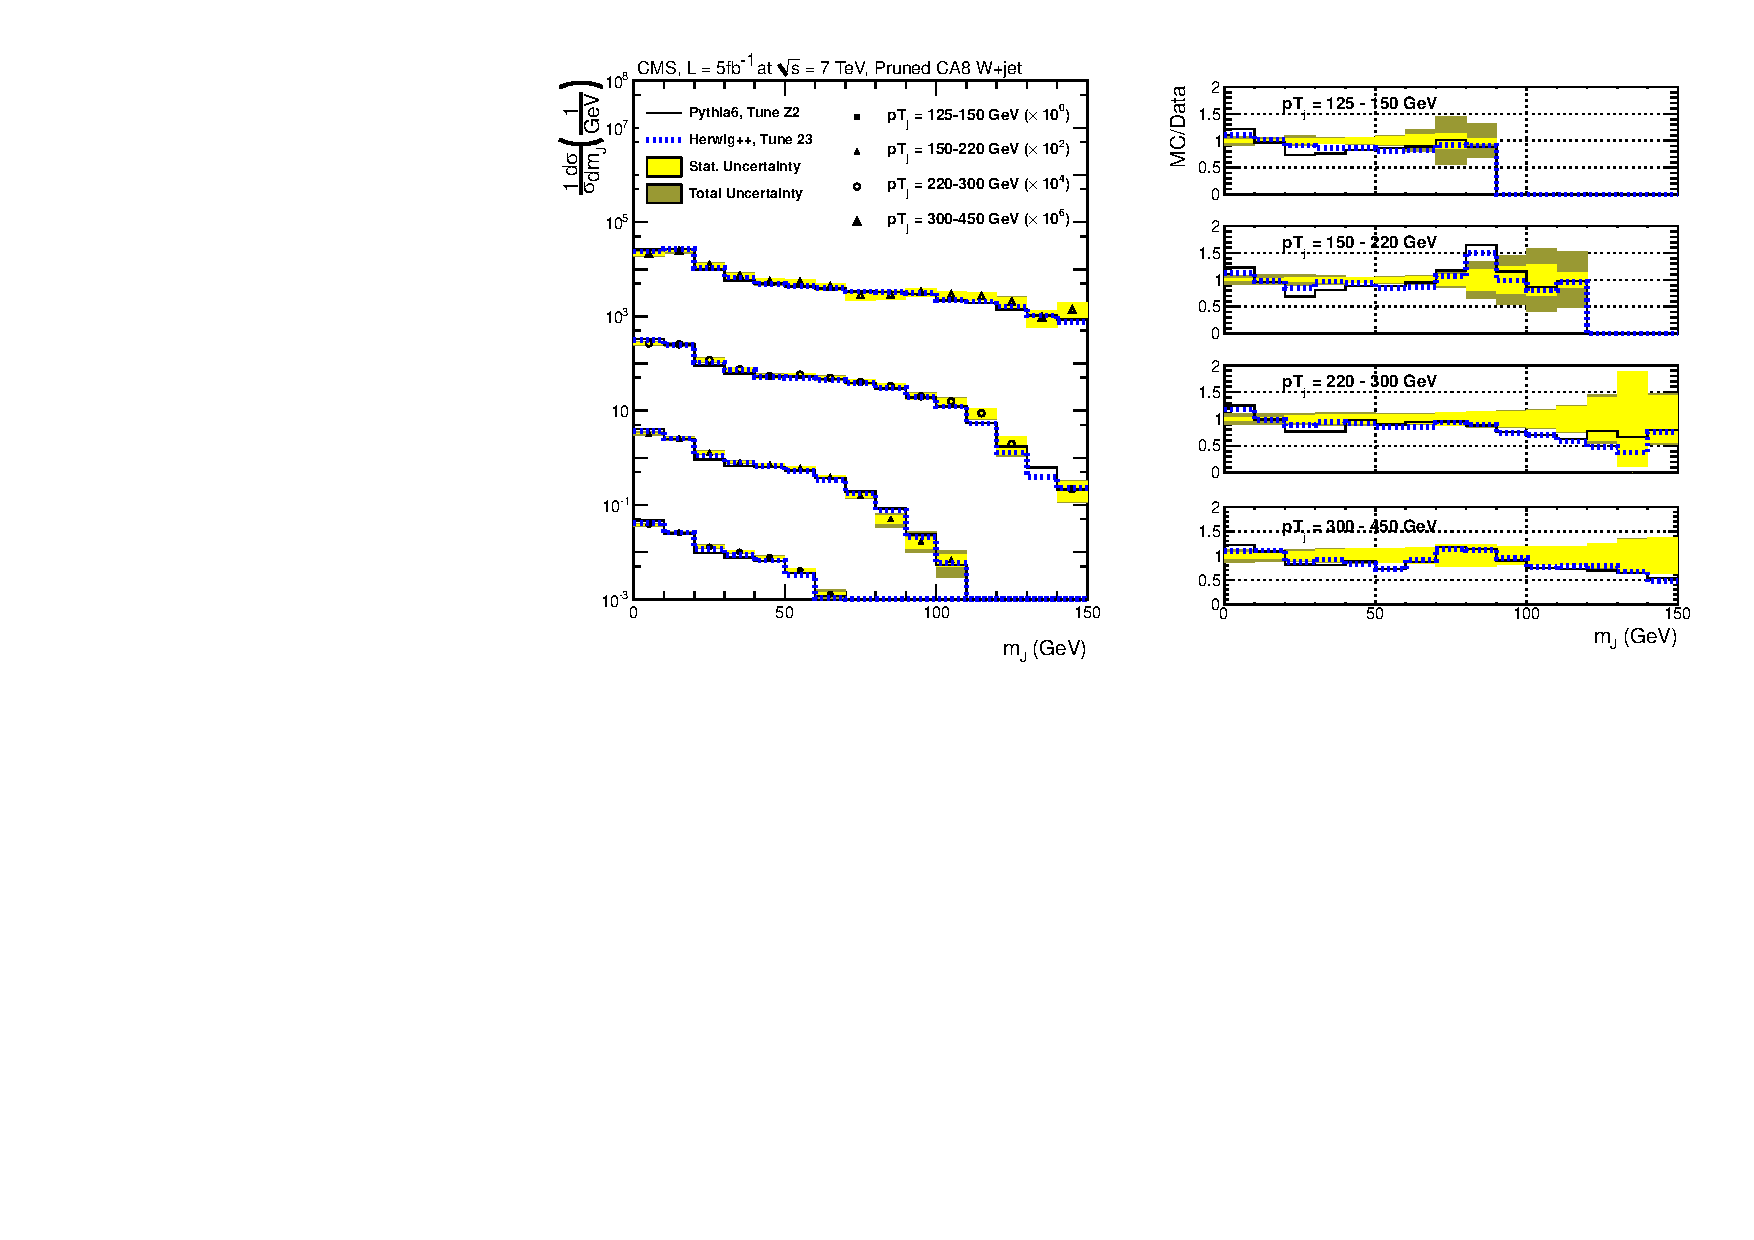
\includegraphics[width=0.99\textwidth]{figs/Wln/jetmassunf_ca8pr_log_W.pdf}
\caption{Distributions in $m_J$ for unfolded, pruned CA8 jets in \PW$(\ell\nu_\ell)$+jet events. The data (black symbols) for different bins in $\pt$ are compared to MC expectations from {\MADGRAPH}+\PYTHIA (solid lines) and \HERWIG (dotted lines) on the left. The ratios of MC to data are given on the right.
The statistical uncertainty is shown in light shading, and the total uncertainty in dark shading.}
\label{figs:prunedWmnInt1}
\end{figure}

\begin{figure}[!htb]
\centering
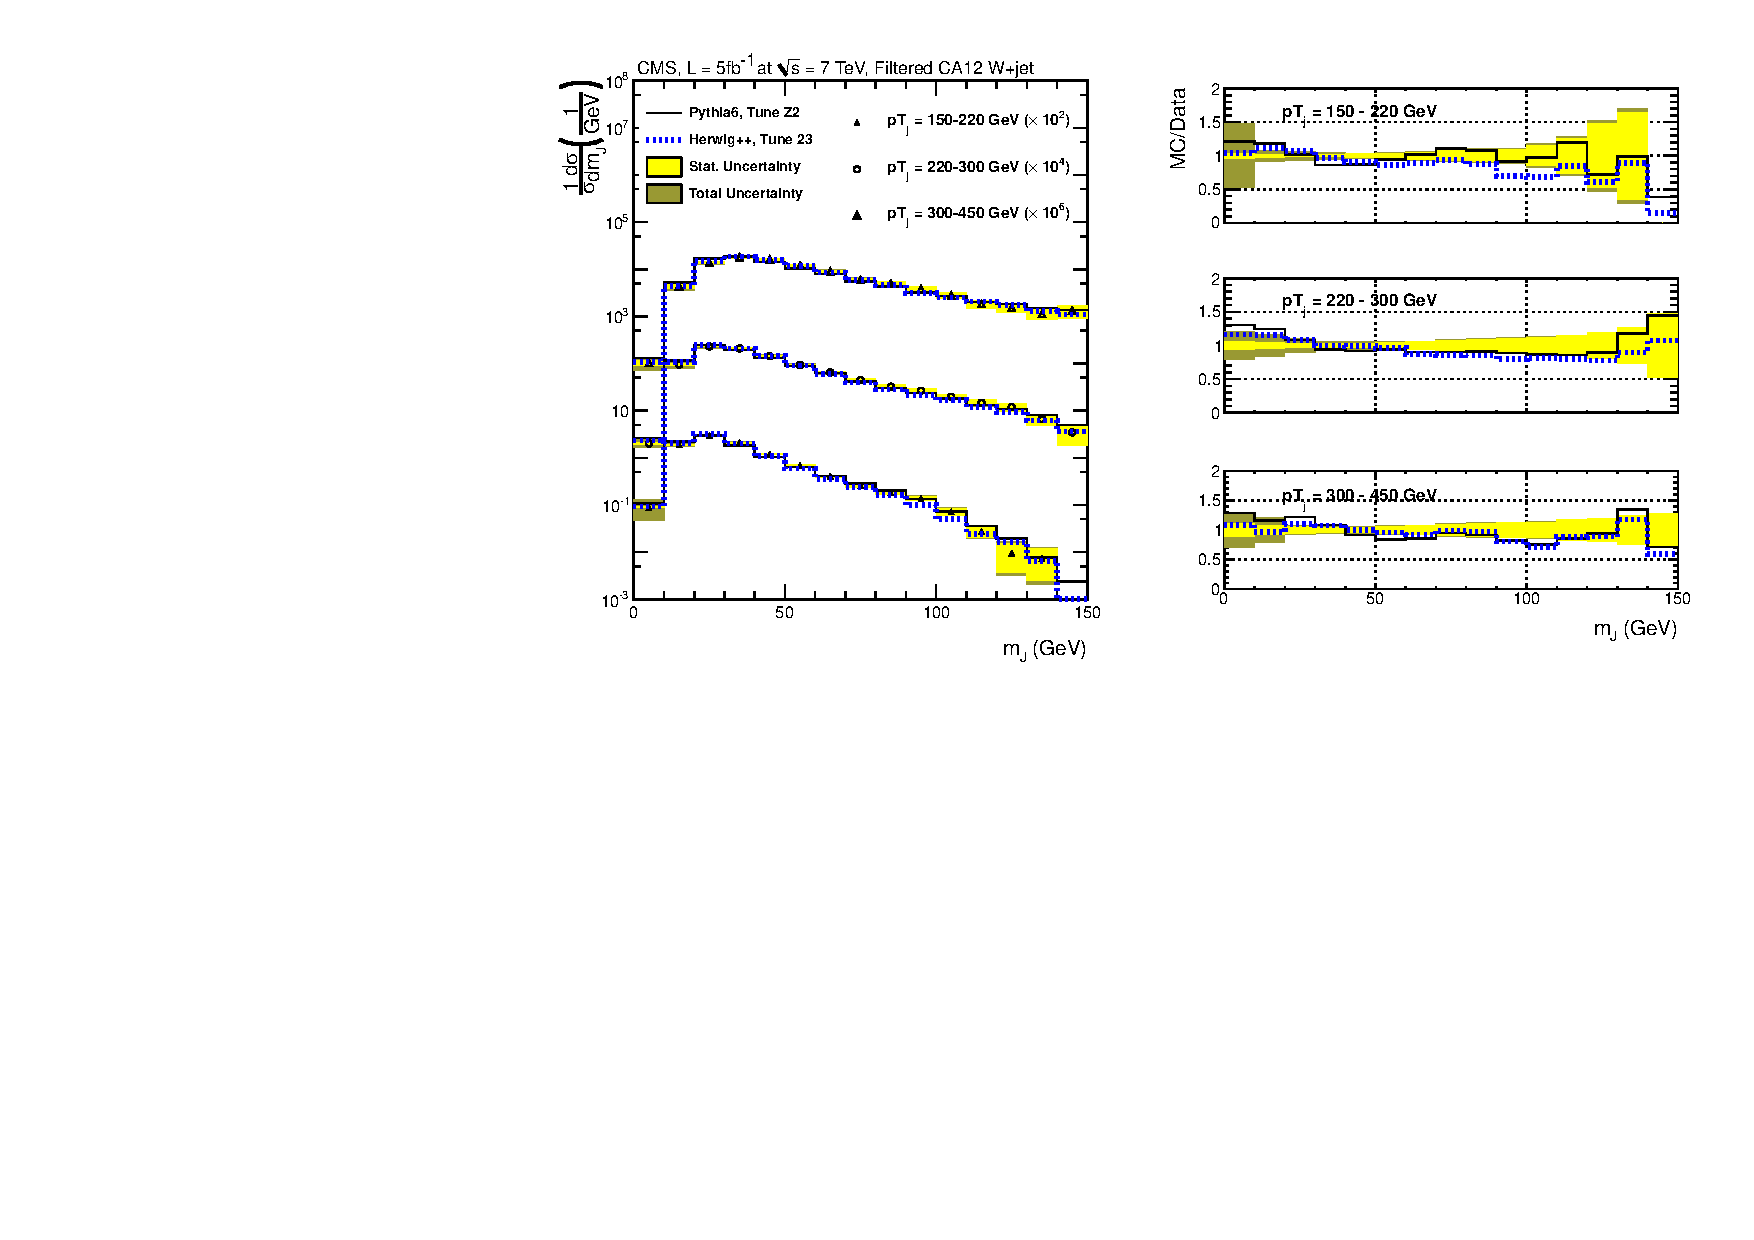
\includegraphics[width=0.99\textwidth]{figs/Wln/jetmassunf_ca12ft_log_W.pdf}
\caption{Distributions in $m_J$ for unfolded, filtered CA12 jets in \PW$(\ell\nu_\ell)$+jet events. The data (black symbols) for different bins in $\pt$ are compared to MC expectations from {\MADGRAPH}+\PYTHIA (solid lines) and \HERWIG (dotted lines) on the left. The ratios of MC to data are given on the right.
The statistical uncertainty is shown in light shading, and the total uncertainty in dark shading.}
\label{figs:prunedWmnInt2}
\end{figure}

\clearpage








\clearpage

\section{Summary}


\bibliography{auto_generated}


